\documentclass[12pt, letterpaper]{report}% "letterpaper" matches US standard paper size.
\setcounter{tocdepth}{3}
% --- PACKAGES: Each one adds a capability to LaTeX ---
% Think of packages like Python imports or C #includes.


% ---------- Page Layout ----------
\usepackage[top=1in,bottom=1in,left=1in,right=1in]{geometry} % geometry lets you set margins. 1-inch all around is standard for reports.
% ---------- Encoding & Fonts ----------
\usepackage[utf8]{inputenc}% Allows special characters (é, ü, °) to be typed directly.
\usepackage[T1]{fontenc} % Ensures proper font encoding in the output PDF. Without this, copy-pasting from the PDF can produce garbled characters.
% ---------- Graphics & Figures ----------
\usepackage{graphicx}% THE core package for inserting images.
% Usage: \includegraphics[width=0.8\textwidth]{filename.png}
\graphicspath{{figures3/}}
\usepackage{float}% Gives you the [H] placement option for figures/tables. [H] means "put it HERE, not where LaTeX thinks is best." Very useful when you need a figure right after the text that references it.
\usepackage{subcaption}% Lets you put multiple images side-by-side in a single figure environment. Example: Figure 3(a) and Figure 3(b) next to each other.
% ---------- Tables ----------
\usepackage{booktabs} % Provides \toprule, \midrule, \bottomrule for professional-looking tables.
% Rule of thumb: NEVER use vertical lines in tables. Use booktabs rules instead.
\usepackage{tabularx}% Adds the tabularx environment, which lets columns auto-expand to fill width. Great for tables that need to span the full page width.
\usepackage{multirow}% Allows cells that span multiple rows in tables.
\usepackage{longtable}% For tables that are too long to fit on one page (like a Bill of Materials).
% ---------- Math ----------
\usepackage{amsmath}% The standard package for equations. Adds align, equation*, etc.
\usepackage{amssymb}% Extra math symbols (e.g., \therefore, \because, \pm).
\usepackage{siunitx}% Proper formatting for SI units.
\sisetup{per-mode=fraction}
\sisetup{exponent-product=\cdot}
\DeclareSIUnit{\fahrenheit}{\degree F}
% Usage: \SI{100}{\celsius}, \SI{10000}{psi}, \SI{10}{\centi\meter}
% This ensures consistent unit formatting throughout the document.
% ---------- Bibliography ----------
\usepackage[numbers, sort&compress]{natbib}
% IEEE-style numeric citations: [1], [2,3], [4-7]
% "sort&compress" turns [3,1,2] into [1-3]
% ---------- Cross-Referencing & Links ----------
\usepackage[
	colorlinks=true,
	linkcolor=blue,      % Internal links (sections, figures)
	citecolor=blue,      % Citation links
	urlcolor=blue         % URL links
]{hyperref}
% Makes all references, citations, and URLs clickable in the PDF.
% Set colorlinks=false if you want boxes instead of colored text.
% ---------- Captions ----------
\usepackage[
	font=small,           % Caption text slightly smaller than body
	labelfont=bf,         % "Figure 1:" is bold
	textfont=it            % The caption description is italic
]{caption}% Makes figure/table captions look more professional.
% ---------- Headers & Footers ----------
\usepackage{fancyhdr}% Customizable headers and footers.
\pagestyle{fancy}% Activate the fancy header/footer style.
\fancyhf{}% Clear all default header/footer content.
\fancyhead[L]{\small Team 16 --- Noble Aggie Labs}% Left header: team name.
\fancyhead[R]{\small EME 185}% Right header: course number.
\fancyfoot[C]{\thepage}% Center footer: page number.
\renewcommand{\headrulewidth}{0.4pt}% Thin line under the header. Set to 0pt to remove.
% ---------- Paragraph Formatting ----------
\usepackage{parskip}% Adds space between paragraphs instead of indenting the first line. This is more common in engineering reports than academic papers.
\setlength{\parindent}{0pt}% Explicitly remove paragraph indentation (parskip should handle this, but belt-and-suspenders doesn't hurt for readability).
% ---------- Line Spacing ----------
\usepackage{setspace}
% \onehalfspacing% 1.5 line spacing is easier to read and mark up than single spacing. Change to \doublespacing if required.
\onehalfspacing
%-------- For Box diagrams
\usepackage{tikz}
\usetikzlibrary{patterns}
\usetikzlibrary{patterns,intersections}
\usetikzlibrary{arrows.meta, positioning}
\usetikzlibrary{shapes.geometric}
\usetikzlibrary{arrows.meta, shapes.geometric, shapes.misc, positioning}
\usetikzlibrary{calc}
% ---------- Appendix Support ----------
\usepackage[title,titletoc,page]{appendix} % Adds "Appendices" header and includes appendices in the Table of Contents. [title, titletoc] ensures they are labeled A, B, C
%----------- Title/Chapter formatting -----------------
\usepackage{titlesec}
% Format \chapter to look simple (no giant text, no separate page)
\usepackage{pdfpages}
% Allows you to insert entire PDF Pages (e.g., for Gantt charts, concept screening matrices) with \includepdf.
\usepackage{geometry}
%allows you to set margins and page size. 
\usepackage{mdframed}     % warning/note boxes, important equations
	\mdfsetup{linewidth=1pt}
\usepackage{enumitem}     % list formatting
\usepackage{booktabs}     % tables
\usepackage{xcolor}       % color support
\usepackage{upgreek}


\definecolor{warnred}{RGB}{180,30,30}
\definecolor{warnbg}{RGB}{255,235,235}
\definecolor{notebg}{RGB}{235,245,255}
\definecolor{noteblue}{RGB}{30,80,160}
\definecolor{ucdgold}{RGB}{207, 184, 124}
\definecolor{ucdblue}{RGB}{0, 40, 85}
\definecolor{sandiablue}{RGB}{0,  174, 214}



\newmdenv[
  linecolor=warnred, backgroundcolor=warnbg,
  linewidth=1.5pt, innerleftmargin=10pt,
  innerrightmargin=10pt, innertopmargin=8pt,
  innerbottommargin=8pt, skipabove=10pt, skipbelow=6pt
]{warningbox}

\newmdenv[
  linecolor=noteblue, backgroundcolor=notebg,
  linewidth=1pt, innerleftmargin=10pt,
  innerrightmargin=10pt, innertopmargin=8pt,
  innerbottommargin=8pt, skipabove=10pt, skipbelow=6pt
]{notebox}


\titleformat{\chapter}
 {\LARGE\bfseries}  % format
 {}                % label
 {0em}                         % sep between label and title
 {}                            % before-code
\titlespacing*{\chapter}{0pt}{20pt}{10pt}  % left, before, after


\makeatletter
\g@addto@macro\appendix{%
 \titleformat{\chapter}[block]
	{\huge\bfseries\centering}
	{\appendixname\ \thechapter}
	{0em}
	{\vspace{0.5em}\\}%
}
\makeatother

% ---------- PDF Metadata ----------
\hypersetup{
    pdftitle={Final Design Report -- Passive Temperature Compensation Device},
    pdfauthor={Team 16: Noble Aggie Labs},
    pdfsubject={EME-185A/B Senior Design, UC Davis}
}
%-----------For landscape pages----------
\usepackage{pdflscape}
\usepackage{pgfplots}
	\pgfplotsset{compat=1.18}
	\usepgfplotslibrary{fillbetween}
	\pgfmathdeclarefunction{normalpdf}{3}{%
    \pgfmathparse{1/(#3*sqrt(2*pi))*exp(-(#1-#2)^2/(2*#3^2))}%
	}
\usepackage{multirow}
\usepackage{array}      % for >{\raggedright\arraybackslash}
\usepackage{makecell}   % for \makecell
\usepackage{calc}
\usepackage{multicol}
\usepackage{wrapfig}
\usepackage{nicefrac}
\usepackage[bottom]{footmisc}

% In your preamble
\newcounter{mycounter}           % creates a counter, initialized to 0
\newcounter{sub}[mycounter]      % resets 'sub' when 'mycounter' increments
% ============================================================================
% SECTION 0.5: CUSTOM COMMANDS (Modular Helpers)
% ============================================================================
% These are reusable shortcuts. Define them once, use them everywhere.
% If a name or term changes, you only edit it in ONE place.


% --- Project-specific shortcuts ---
\newcommand{\projecttitle}{Passive Temperature Compensation Device}
\newcommand{\teamname}{Noble Aggie Labs}
\newcommand{\teamnumber}{16}
\newcommand{\sponsor}{Dr.\ Bradley Bon}
\newcommand{\organization}{Sandia National Laboratories}
\newcommand{\coursename}{EME 185}
\newcommand{\instructor}{Professor Jonathon Schofield}
\newcommand{\university}{University of California, Davis}
\newcommand{\ta}{Teaching Assistant Xiangpu Wang}
\newcommand{\duedate}{5 June 2026}
% --- Convenience commands for common terms ---
% Using these ensures consistent terminology throughout the report.
\newcommand{\device}{PTCD}
\newcommand{\degC}{^{\circ}\text{C}}    % Degree Celsius symbol, properly formatted
\newcommand{\requiredRelationship}{D_{\text{effective}} = A_1 (T_{\text{ambient}} - T_{\text{reference}}) + A_0}
\newcommand{\transferFunction}{D_{\text{eff}}=\frac{dD_{\text{eff}}}{dX} \left[\frac{dL}{dT}\frac{dX}{dL}(T-T_{\text{ref}})+X\left(T_{\text{ref}} \right) \right]}

\newcommand{\Dcoldval}{}
\newcommand{\Dcold}{D_{\text{effective}}(\SI{-60}{\celsius}) = 383.5 \pm \SI{19.2}{\micro\meter}}
\newcommand{\Dhot}{D_{\text{effective}}(\SI{80}{\celsius}) = 170.2 \pm \SI{16.9}{\micro\meter}}
\newcommand{\Dref}{D_{\text{effective}}(\SI{25}{\celsius}) = 292.1 \pm \SI{12.7}{\micro\meter}}

\newcommand{\Thot}{\SI{80}{\degreeCelsius}} %Celcius
\newcommand{\Tcold}{\SI{-60}{\degreeCelsius}} %Celcius
\newcommand{\Tref}{\SI{25}{\degreeCelsius}} %Celcius
\newcommand{\specTempChange}{\SI{140}{\degreeCelsius}}

\newcommand{\specEAl}{\SI{68.95}{\giga \pascal}}
\newcommand{\specEALLV}{\SI{55}{\giga \pascal}}
\newcommand{\specEInv}{\SI{141}{\giga \pascal}}
\newcommand{\specEInc}{\SI{200}{\giga \pascal}}
\newcommand{\specActuatorCTE}{\SI{22.85}{\micro\meter\per\meter\per\celsius}} %Evaluated at 25C
\newcommand{\specMountCTE}{\SI{-30}{\micro\meter\per\meter\per\celsius}}
\newcommand{\specInvarCTE}{\SI{1.3}{\micro\meter\per\meter\per\celsius}}
\newcommand{\specInconelCTE}{\SI{13.2}{\micro\meter\per\meter\per\celsius}}
\newcommand{\specBellowsK}{\SI{75.3}{\kilo \newton \per \meter}} % 430 lb/in
\newcommand{\specBellowsHeight}{\SI{22.86}{\milli \meter}} % = Neck 1 length + Neck 2 length + Conv free diameter = 2*(0.07") + 0.76"
\newcommand{\specBellowsOD}{\SI{6.528}{\milli \meter}} % Conv OD 0.257"
\newcommand{\specBellowsID}{\SI{3.353}{\milli \meter}} % Conv ID 0.132"
\newcommand{\specBellowsSquirm}{\SI{20.68}{\mega \pascal}} % 3000 psi
\newcommand{\specBellowsBurst}{\SI{74.12}{\mega \pascal}} % 10750 psi

\newcommand{\Xhot}{\SI{480.696}{\micro \meter}}
\newcommand{\Xcold}{\SI{213.289}{\micro \meter}}
\newcommand{\specLengthChange}{\SI{267.407}{\micro \meter}}
\newcommand{\govErrorProp}{u_x = \sqrt{\frac{\pi(\sigma_x^2+\sigma_y^2)}{2}}}
\newcommand{\govActuator}{\Delta L = L_0 \Delta T \alpha}
\newcommand{\govValve}{D_{\text{eff}} = \sqrt{\frac{2}{\pi}}}
\newcommand{\specPressure}{\SI{68.95}{\mega \pascal}}%  68.94757 MPa
\newcommand{\AoneExact}{\SI{-1.524e-3}{\milli\meter\per\celsius}}
\newcommand{\Aone}{\AoneExact \pm 5\%}
\newcommand{\AzeroExact}{\SI{0.254}{\milli\meter}}
\newcommand{\Azero}{\AzeroExact \pm 5\%}
\newcommand{\imageHeight}{4in} % Default image height for figures. Adjust as needed.
\newcommand{\specCrossSectArea}{\SI{6.3e-5}{\meter \squared}}
\newcommand{\specOrigActuatorLength}{\SI{32.991}{\milli \meter}}
\newcommand{\specActDefTotal}{\SI{267}{\micro \meter}}
\newcommand{\specActDefHot}{\SI{152.8}{\micro \meter}}

% TF Force Balance Matrix (given as an escaped command because it is given twice in the report)

\newcommand{\forceMatrix}
{
	\begin{bmatrix}
		k_M & k_A  & 0    & 0     & 0     & 0     & 0     & 0     \\
		0   & k_A  & -k_S & 0     & 0     & 0     & 0     & 0     \\
		k_M & 0    & 0    & 0     & 0     & 0     & 0     & -k_W  \\
		0   & 0    & 0    & -k_T  & 0     & 0     & -k_H  & k_W   \\
		0   & 0    & 0    & 0     & -k_B  & k_V   & 0     & 0     \\
		0   & 0    & 0    & 0     & k_B   & 0     & k_H   & 0     \\
		1   & -1   & -1   & 1     & 0     & 0     & 0     & 1    \\
		0   & 0    & 0    & 1     & 1     & 1     & -1    & 0
	\end{bmatrix}
	\begin{bmatrix}
		L_M \\ L_A \\ L_S \\ L_T \\ L_B \\ L_V \\ L_H \\ L_W
	\end{bmatrix}
	=
	\begin{bmatrix}
		k_M \ell_M + k_A \ell_A \\
		k_A \ell_A - k_S \ell_S \\
		k_M \ell_M - k_W \ell_W \\
		k_W \ell_W - k_T \ell_T - k_H \ell_H \\
		k_V \ell_V - k_B \ell_B \\
		k_H \ell_H + k_B \ell_B \\
		0 \\
		0
	\end{bmatrix}
}

% Transfer function specifications

\newcommand{\GA}{\SI{1.91}{\micro\meter\per\celsius}}
\newcommand{\GV}{\num{-0.798}}

\newcommand{\ReqA}{The device shall passively restrict gas flow according to the Required Relationship $D = A_1 \Delta T + A_0$}
\newcommand{\ReqB}{The device should remain within a \SI{10}{\centi\meter} $\times$ \SI{10}{\centi\meter} $\times$ \SI{10}{\centi\meter} mechanical envelope}
\newcommand{\ReqC}{The device shall restrict Hydrogen at \specPressure\ and $T_{amb} + 20 \degC$ for 60 seconds in compliance with requirement R.1}
\newcommand{\RRfull}
{
	\begin{equation}
		\begin{aligned}
			D_{eff} &= \hat{G}_{V_0} \hat{G}_{A_0} \Delta T + D_{ref} \\
			&= \frac{dD}{dL} \frac{dL}{dT} (T_{amb} - T_{ref}) + D(T_{ref}) \\
			&= A_1 \Delta T + A_0
		\end{aligned}
	\end{equation}
}

% Valve specifications
\newcommand{\SpecVAA}{The valve subsystem shall passively control the effective orifice diameter as directly driven by the actuator at a conversion rate of $\frac{dD}{dL} = \GV$}
\newcommand{\SpecVAB}{The valve subsystem shall define the reference effective orifice diameter}
\newcommand{\SpecVABapp}{$D_{eff}(T_{ref}) = \AzeroExact$}
\newcommand{\SpecVB}{The valve subsystem shall not exceed a \SI{10}{\centi\meter} $\times$ \SI{5}{\centi\meter} $\times$ \SI{10}{\centi\meter} mechanical envelope}
\newcommand{\SpecVCA}{The housing shall withstand an internal pressure of \specPressure}
\newcommand{\SpecVCB}{Wetted components shall maintain a hermetic seal at this pressure}
\newcommand{\SpecVCC}{Wetted components shall not permit Hydrogen diffusion or embrittlement}

% Actuator specifications
\newcommand{\SpecAAA}{The actuator subsystem shall passively drive the valve subsystem in response to ambient temperature at a rate of $\frac{dL}{dT} = \GA$}
\newcommand{\SpecAAB}{The actuator subsystem shall facilitate user calibration of the device}
\newcommand{\SpecAB}{The actuator subsystem shall not exceed a \SI{10}{\centi\meter} $\times$ \SI{5}{\centi\meter} $\times$ \SI{10}{\centi\meter} mechanical envelope}
\newcommand{\SpecACA}{The actuator shall allow no more than \textbf{\textcolor{red}{[TODO: Spec Temp]}} deviation in its temperature from $T_{amb}$\ within the test window}

% --- Figure insertion helper ---
% This command simplifies inserting a figure with a caption and label.
% Usage: \insertfigure{width}{filename}{caption text}{fig:label}
%
% Parameters:
%   #1 = width relative to text width (e.g., 0.8 for 80%)
%   #2 = filename (without path if images are in the same directory)
%   #3 = caption text
%   #4 = label for cross-referencing (use fig:prefix by convention)
\newcommand{\insertfigure}[4]{%
	\begin{figure}[H]
		\centering
		\includegraphics[width=#1\textwidth]{#2}
		\caption{#3}
		\label{#4}
	\end{figure}
}

% --- TODO marker for draft mode ---
% Prints a bold red "TODO" so you can easily spot incomplete sections.
\usepackage{xcolor}
\usepackage{tocloft} % For listoftodos
% --- TODO marker ---
\newlistof{todos}{tod}{List of TODO's}
\newcommand{\todo}[1]{%
    \textbf{\textcolor{red}{[TODO: #1]}}%
    \addcontentsline{tod}{todos}{\protect\numberline{\thepage}#1}%
}

% For links to spec table
\newcommand{\specref}[1]{\hyperref[tab:specs]{#1}}

\usepackage{lmodern} % DELETE BEFORE SUBMISSION; this is to help the pdf render more easily.


% ============================================================================
% BEGIN DOCUMENT
% ============================================================================

\begin{document}

\chapter{Requirement Satisfaction}
\label{chap:sat}

	

	\section{Error Analysis}
	\label{sec:sat:error}

	\section{System Transfer Function}
	\label{sec:sat:TF}

		The required transfer function from Section~\ref{subsec:intro:specs:RR} describes the system under ideal conditions and cannot properly account for systematic errors.
		To fully analyze the expected performance of the \device, a new, comprehensive system Transfer Function must be derived that can be compared to the required output: 

		\begin{equation}
			\hat{G}_{sys} = A_1 (T-T_{ref}) + A_0 = (\Aone)(T-T_{ref}) + (\Azero)
			\label{eq:req_TF}
		\end{equation}

		This section presents a full derivation of this transfer function, represented in block-diagram form on the following page:
		% \newpage
		% \todo{Uncomment pdf. It may throw some errors.}
		% \newpage
		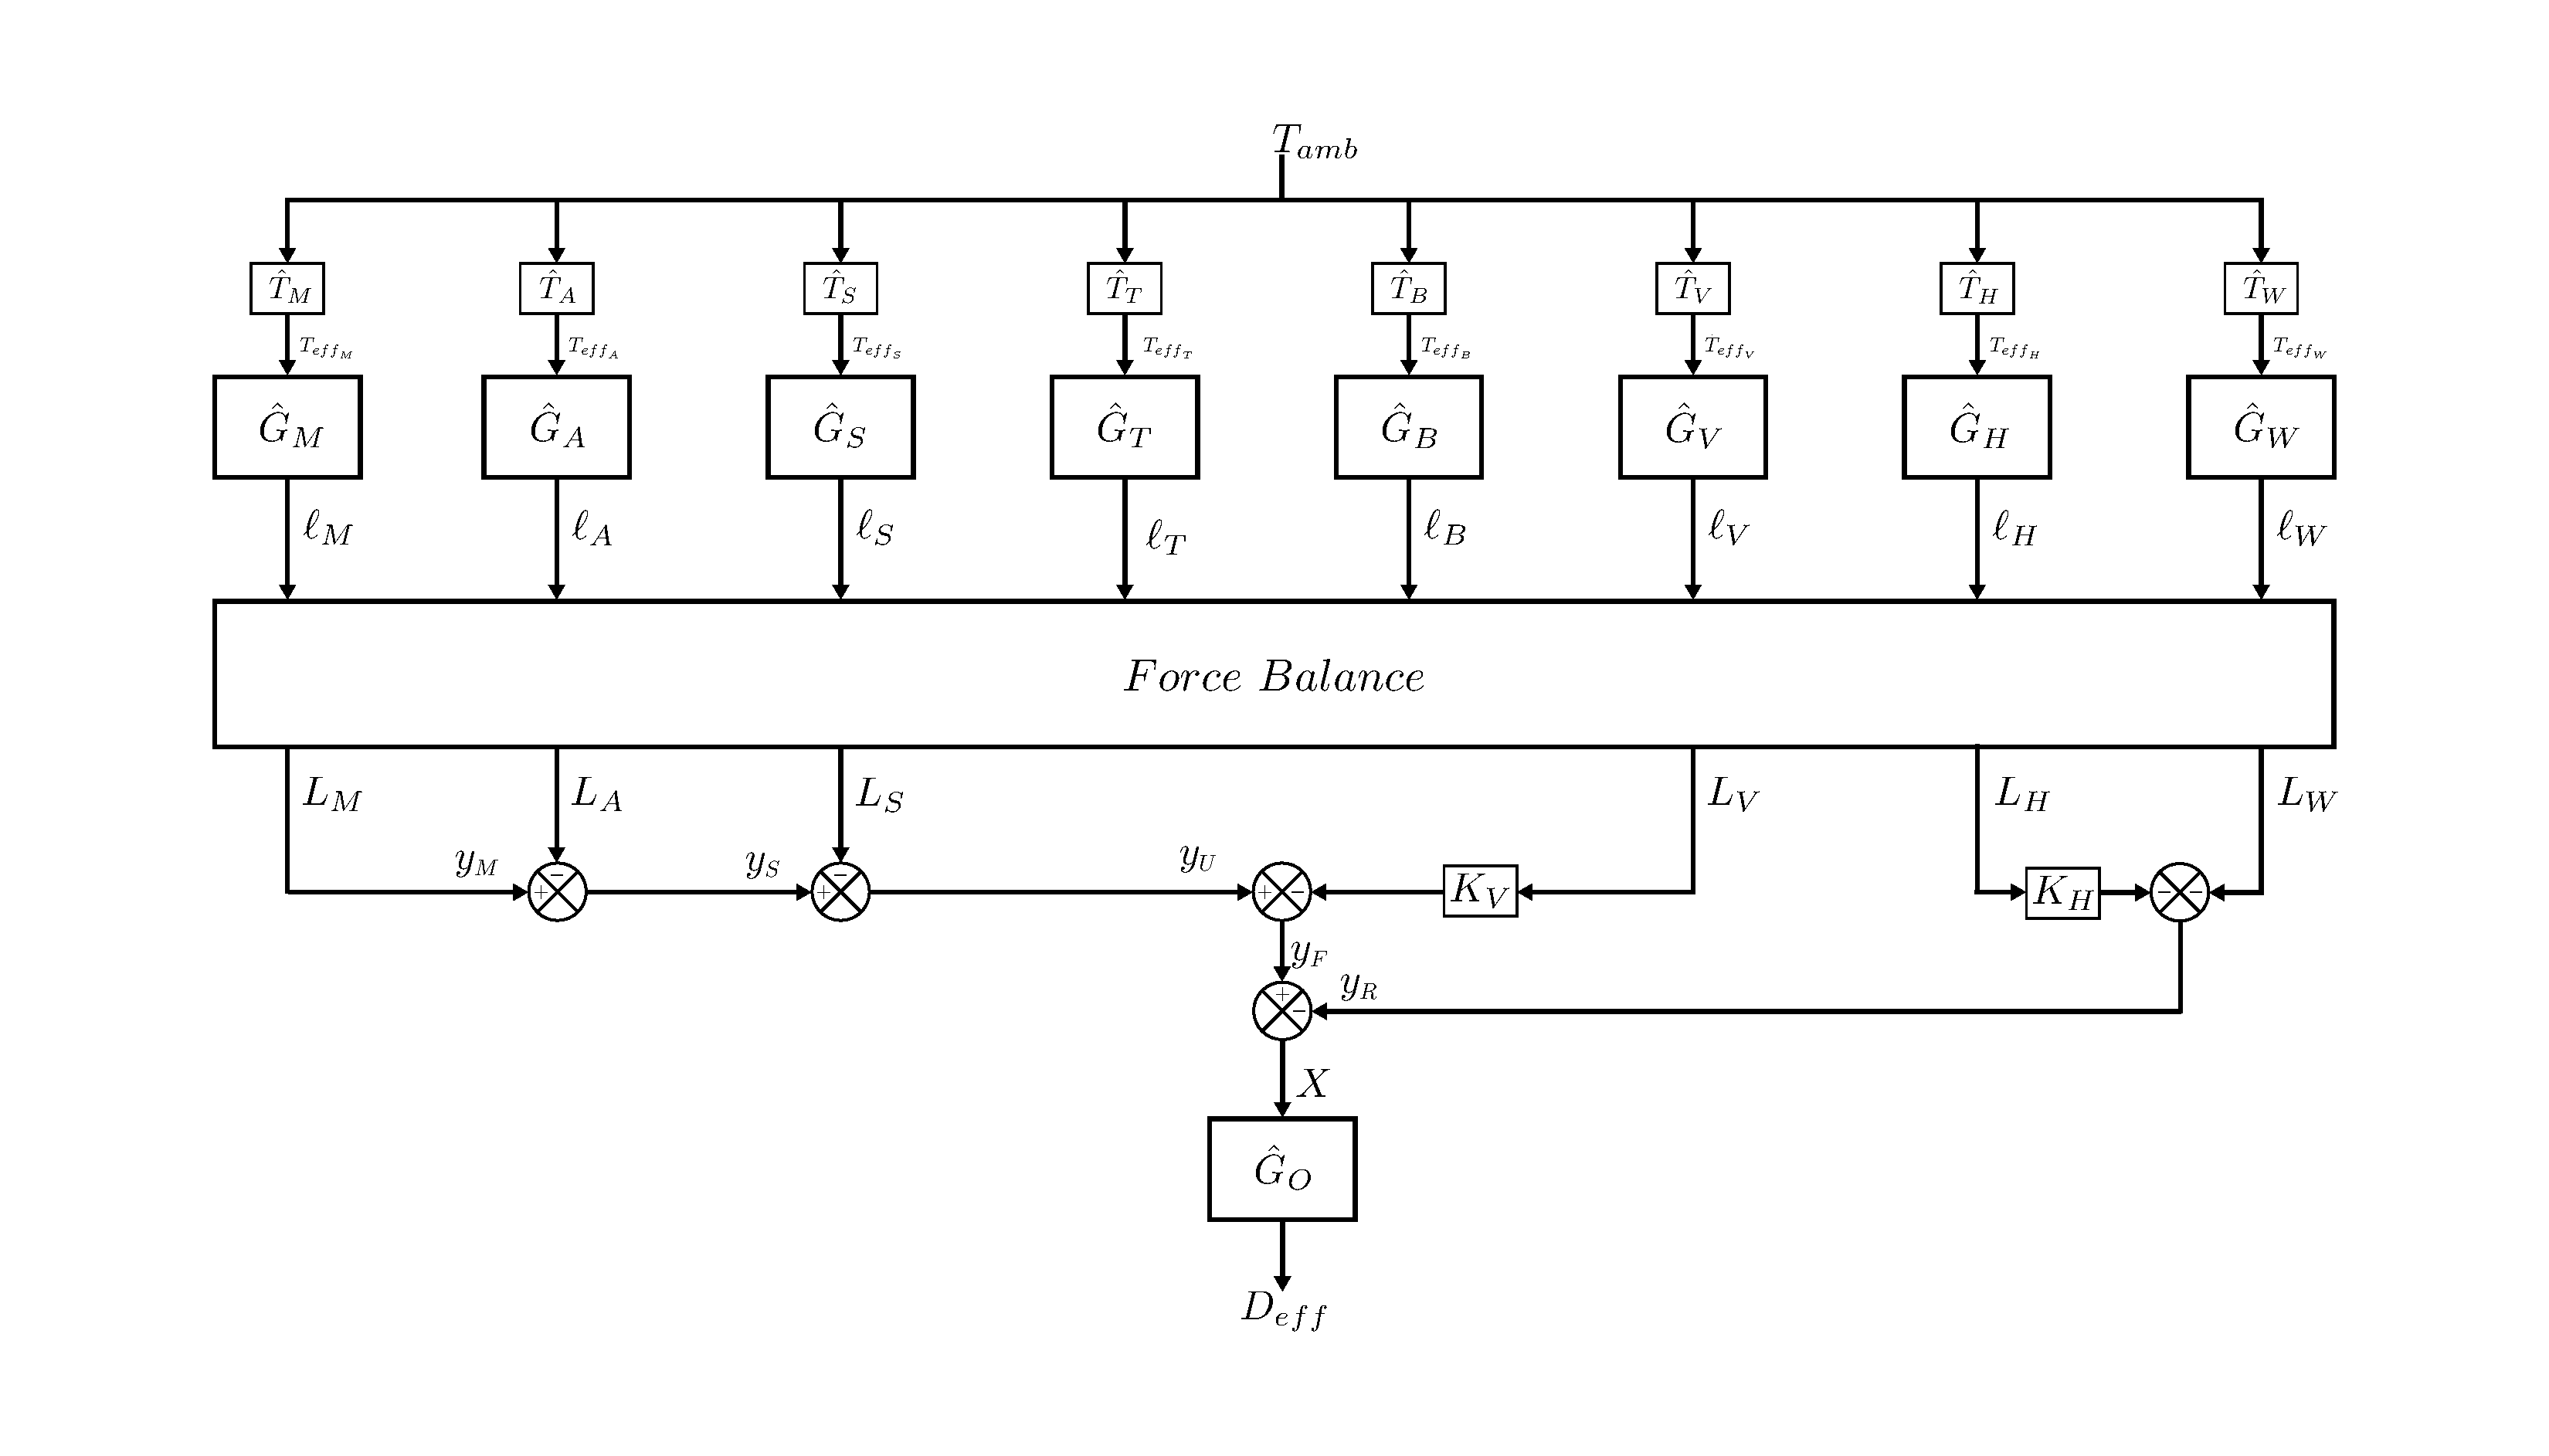
\includepdf[pages=1, fitpaper=true, landscape=true]{pdf/TF_import.pdf}

		The \device\ System Transfer Function comprises 21 smaller independent transfer functions whose respective output values are summed and equated in accordance with the physical behavior of the system.
		Its details will take a moment to unpack.

		First, notice the general structure: the transfer function receives $T_{ambient}$ and returns $D_{effective}$ as prescribed.
		The smaller, top $(\hat{T})$ row of sub-transfer functions adjusts $T_{amb}$ for each part in the assembly to account for heat transfer from the hot internal gas.
		The larger, second $(\hat{G})$ row represents the thermal expansion of each dimensionally critical component; each function takes the given adjusted temperature and outputs the thermally expanded length $\ell$ of its respective part.
		However, because the bellows apply a spring force against the actuation motion, these parts will deform slightly. A Force Balance processes these undeformed length values through a system of linear equations, yielding the final length $L$ of each component.
		These final values are summed to obtain the position $y$ of each of the two square holes. Taking the difference between these positions, we obtain the height $X$ of the square orifice, which is finally converted to $D_{effective}$ by the orifice transfer function $\hat{G}_O$.
		
		To understand the origin of the transfer function structure, we must decompose the functional structure of each component of the \device.
		Figure~\ref{fig:positional_block_diagram} illustrates the relative position of each component in simplified fashion.
		Each part's temperature adjustment function $\hat{T}$, thermal transfer function $\hat{G}$, undeformed length $\ell$, and final length $L$ is labeled with its respective subscript as shown in the figure:
		
		\begin{multicols}{2}
			\begin{itemize}
				\item Mount (M)
				\item Actuator (A)
				\item Upper valve stem (S)
				\item Upper "top" bellows (T)
				\item Lower "bottom" bellows (B)
				\item Valve orifice (V)
				\item Housing side walls (H)
				\item Housing top face or "wall" (W)
			\end{itemize}
		\end{multicols}
				
		\begin{figure}[H]
			\centering
			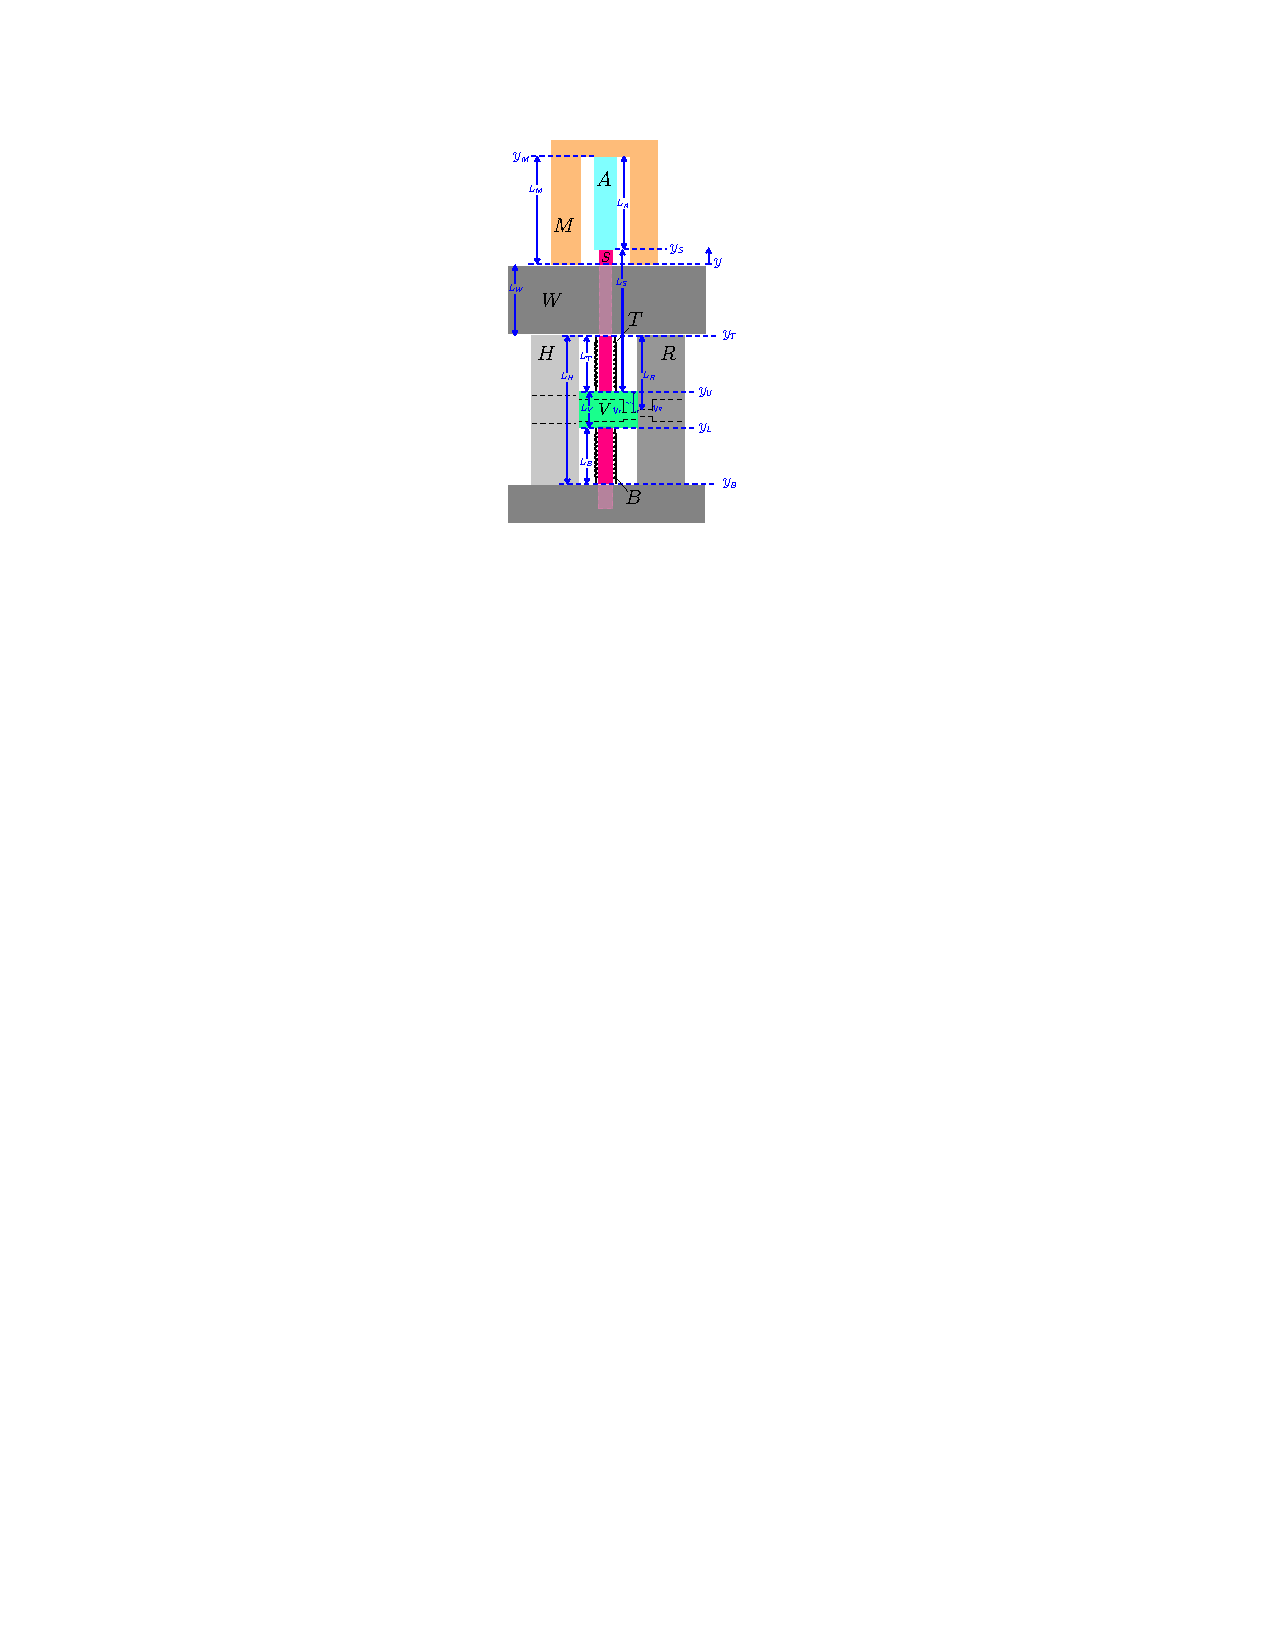
\includegraphics[height=\textheight, width=\textwidth, keepaspectratio]{positional_block_diagram.png}
			\caption{Positional block diagram}
			\label{fig:positional_block_diagram}
		\end{figure}
		
		
		\begin{multicols}{2}
			\begin{figure}[H]
				\centering
				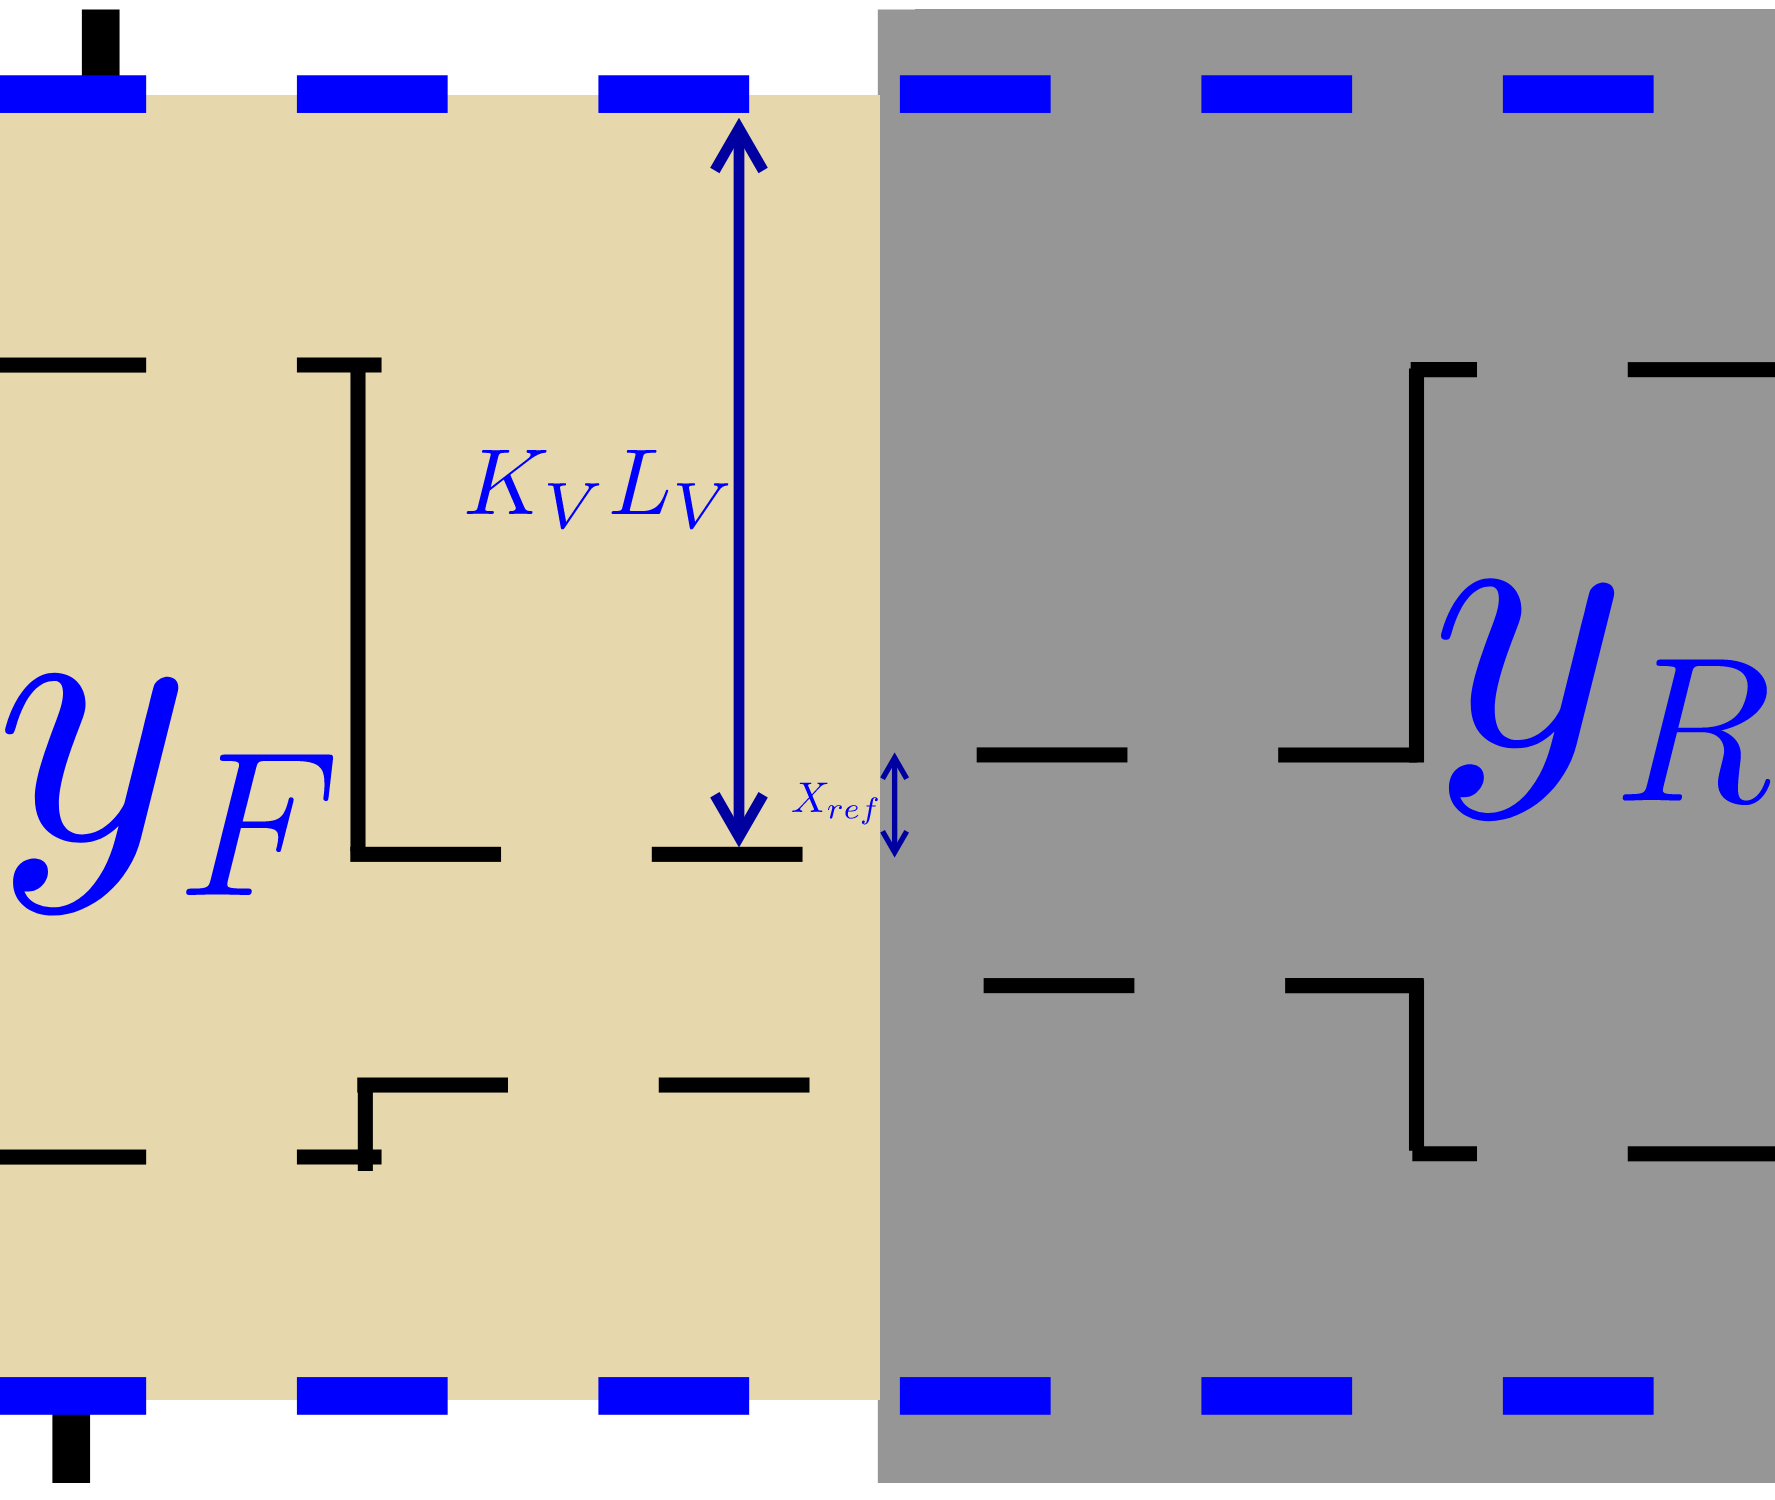
\includegraphics[width=.45\textwidth]{positional_block_diagram_zoom.png}
				\caption{Positional block diagram, detail view}
				\label{fig:positional_block_diagram_zoom}
			\end{figure}

			\begin{figure}[H]
				\centering
				\includegraphics[width=.45\textwidth]{Housing_split.png}
				\caption{Separation between Housing Wall (W) and Housing Body (H)}
				\label{fig:housing_split}
			\end{figure}

			\columnbreak
			
			Figure~\ref{fig:positional_block_diagram_zoom} shows a detail view of certain dimensions around the orifice that will be used later.
			As described in Chapter~\ref{chap:design}, the mount $(M)$ sits atop the housing.
			The actuator $(A)$ dangles from the upper interior surface of the housing center, which for our purposes is defined as the undersurface of the belleville washer.
			The upper valve stem $(S)$ hangs from the bottom of the actuator, passes through the housing wall, and suspends the valve orifice $(V)$, which slides freely against the two surfaces $H$ and $R$.
			Treating the three housing components as a single part, which is realistic because they are electron-beam welded at every seam, the housing "wall" $(W)$ is defined as the top \SI{10}{\milli\meter} of the whole housing assembly (parts V1, V2, and V3) as shown in Figure~\ref{fig:housing_split}.
			The housing body $(H)$ and "rear" $(R)$ share the lower portion shown in the figure; their expansion is coupled.
			These represent the side walls of the housing and behave identically; thus, their behavior is summed by the $H$ term in several calculatiosn.
			The two bellows $(T \text{ and } B)$ span the distance between the valve orifice and the upper and lower housing walls (part V2).
			
			Figure~\ref{fig:positional_block_diagram} also defines several useful positions according to a vertical coordinate frame. The position variable $y$ originates (i.e. equals $0$) at the top surface of the housing, which is considered fixed, and increases vertically.
			Thus, $y_M$ is positive, whereas $y_T$ is negative.
		\end{multicols}

		\subsection{Heat Transfer}
		\label{subsec:sat:TF:dT}

			\todo{Briefly explain new effective temperatures}

		\subsection{Thermal Expansion}
		\label{subsec:sat:TF:top_row}
		Let us forgo the top row of temperature-adjusting functions for now and assume we know the temperature of each part. A full thermal analysis will provide these values later in this report.
		Each of the nine sub-transfer functions along the second row computes the thermal espansion of each part shown in Figure~\ref{fig:positional_block_diagram}.
		Its value can be approximated as a first-order Taylor Expansion\cite{ref_Jensen}\cite{ref_Stewart} with very little error due to the linear behavior of thermal expansion. This yields

				\begin{equation}
					\ell_i = \hat{G}_{thermal} = \ell_0(1 + \frac{d \ell}{dT} \Delta T)
				\end{equation}

			where $\hat{G}_{thermal}$ outputs the expanded dimension $\ell_i$ of part $i$, $\ell_0$ is its machined dimension, and $\Delta T = (T_{amb} - T_{ref})$.
			According to the general principle of thermal expansion\cite[Eq.~4-4]{ref_Hibbeler}, $\frac{d \ell}{dT} = \alpha \ell_0$ where $\alpha$ is the material coefficient of thermal expansion (CTE).
			Thus, the thermal-expansion transfer functions are defined as follows:

			\vspace{1em}
			\begin{mdframed}[userdefinedwidth=\dimexpr\textwidth+1cm\relax, leftmargin=-0.5cm]
				\begin{multicols}{2}

					\begin{align}
						\hat{G}_M &= \ell_{M_0} (1 + \alpha_{ALLV} \left( T_{{eff}_M} - T_{ref} \right) ) \label{eq:G_therm_1}\\
						\hat{G}_A &= \ell_{A_0} (1 + \alpha_{Al} \left( T_{{eff}_A} - T_{ref} \right) ) \\
						\hat{G}_S &= \ell_{S_0} (1 + \alpha_{Inv} \left( T_{{eff}_S} - T_{ref} \right) ) \\
						\hat{G}_T &= \ell_{T_0} (1 + \alpha_{Inc} \left( T_{{eff}_T} - T_{ref} \right) )
					\end{align}
					
					\columnbreak
					
					\begin{align}
						\hat{G}_B &= \ell_{B_0} (1 + \alpha_{Inc} \left( T_{{eff}_B} - T_{ref} \right) ) \\
						\hat{G}_V &= \ell_{V_0} (1 + \alpha_{Inv} \left( T_{{eff}_V} - T_{ref} \right) ) \\
						\hat{G}_H &= \ell_{H_0} (1 + \alpha_{Inv} \left( T_{{eff}_H} - T_{ref} \right) ) \\
						\hat{G}_W &= \ell_{W_0} (1 + \alpha_{Inv} \left( T_{{eff}_W} - T_{ref} \right) ) \label{eq:G_therm_last}
					\end{align}

				\end{multicols}
			\end{mdframed}

			where the material expansion coefficients and machined lengths are shown in Appendix~\ref{app:calcs:TF:G_therm}.

			This yields nine undeformed lengths, helping us to define the positions of each part of the orifice.
			The CTE of aluminum is computed as a function of temperature as defined in Section~\ref{subsec:sat:error:CTE} to find the impact of this error on the final output.
			Dimensional errors are stochastically added or subtracted to each machined part length $\ell_0$. This process is discussed in more detail in Section~\ref{sec:sat:TF:results}. 
			Before this can be calculated, however, the spring reaction of bellows must be reconciled.

		\subsection{Force Balance}
		\label{subsec:sat:TF:force_balance}

			Assuming the \device\ is assembled at $T_{ref}$, which is room temperature, each component is undeformed at that temperature. Thus, $L_i(T_{ref}) = \ell_i(T_{ref})$.
			As the temperature changes, the system behaves as a spring mechanism. The arrangement is shown in Figure~\ref{fig:springs}.

			\begin{figure}[H]
				\centering
				\begin{minipage}{.45\textwidth}
					\centering
					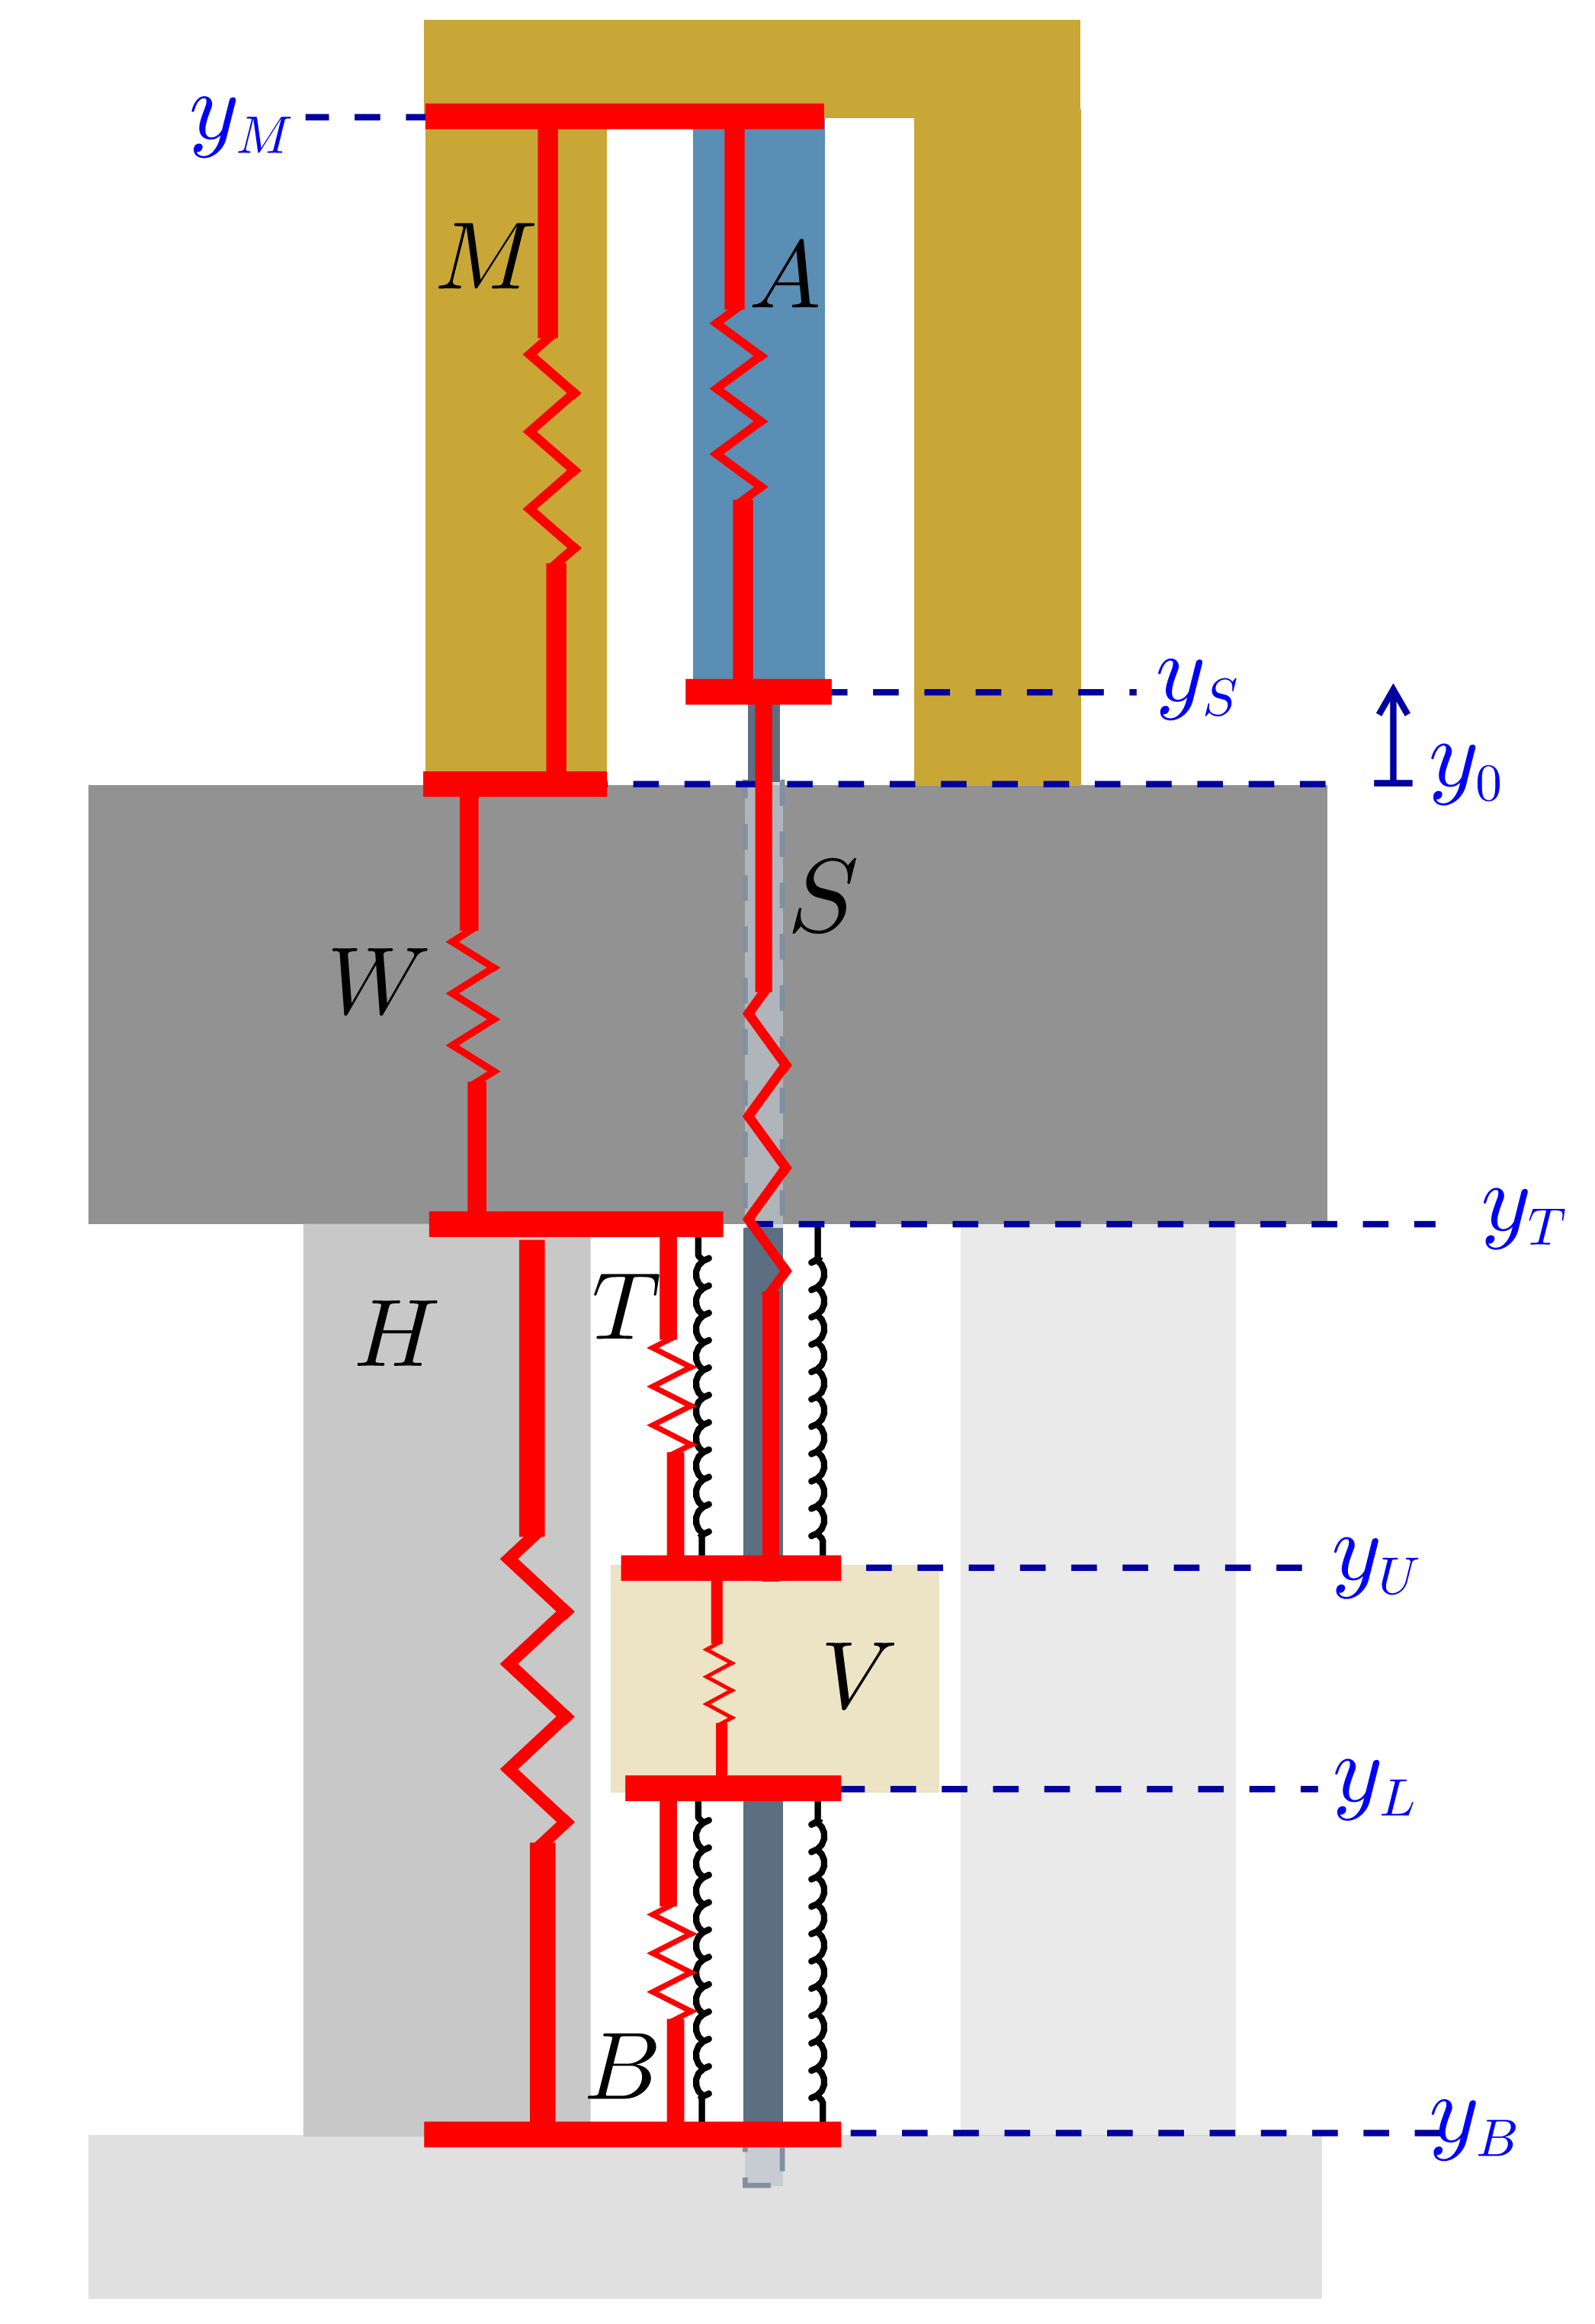
\includegraphics[height=.5\textheight]{springs.png}
					\subcaption{\device\ spring mechanism}
					\label{fig:springs_full}
				\end{minipage}
				\hfill
				\begin{minipage}{.45\textwidth}
					\centering
					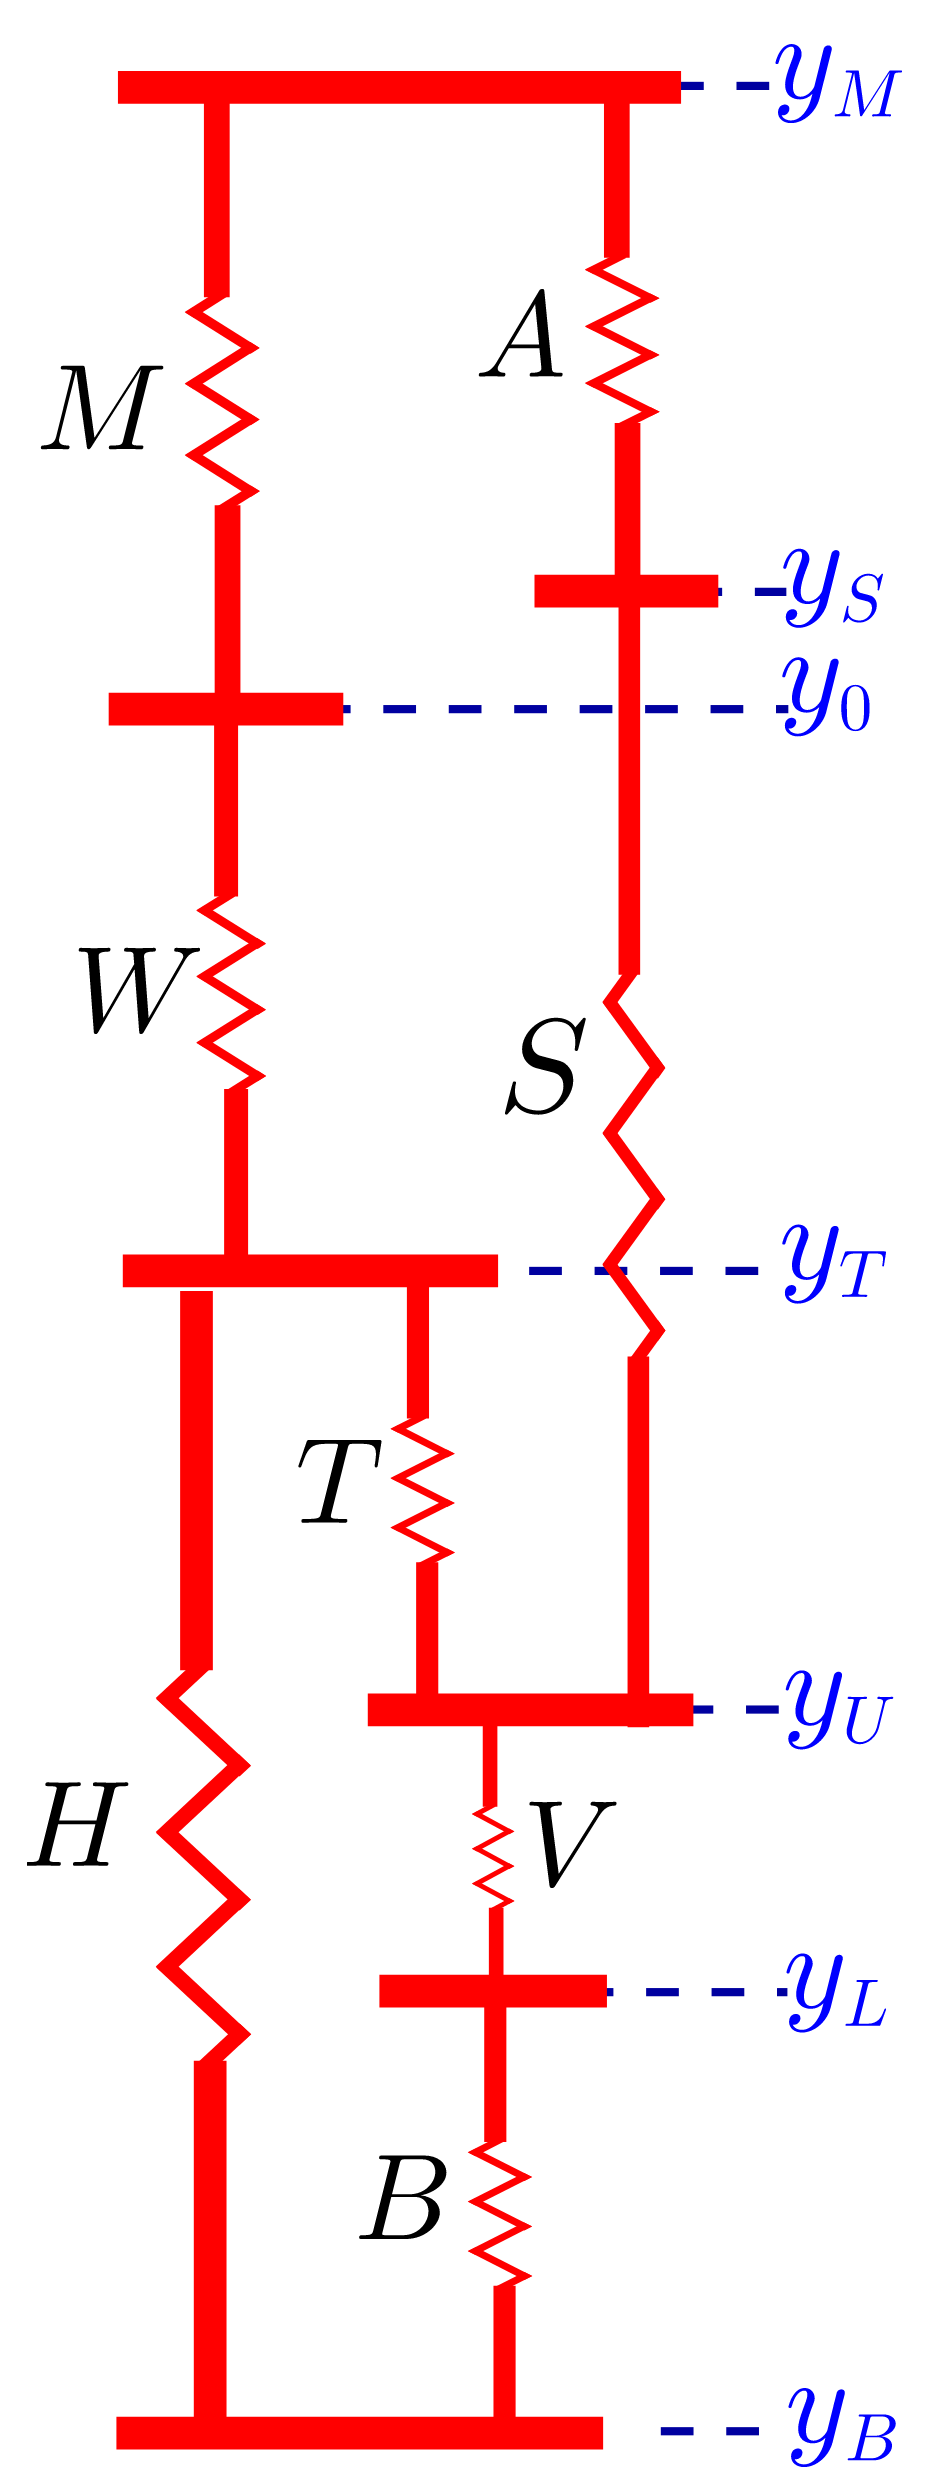
\includegraphics[height=.5\textheight]{springs_simp.png}
					\subcaption{\device\ spring mechanism, simplified}
					\label{fig:springs_simp}
				\end{minipage}
				\caption{Spring deflection}
				\label{fig:springs}
			\end{figure}

			Application of a sum of forces at each node yields a system of eight equations that can be numerically solved to obtain the final deformed length of each part in terms of their spring constants $k$:

			\vspace{1em}
			\begin{mdframed}
				\begin{equation}
					\forceMatrix
					\label{eq:matrix}
				\end{equation}
			\end{mdframed}

			Derivation of this matrix and of its spring constants can be found in Appendix~\ref{app:calcs:TF:force_balance}.
						
		\subsection{Position calculations}
		\label{subsec:sat:TF:pos}

			Finally, we can use these lengths to calculate the values $y_F$ and $y_R$ of the two orifice components shown in Figure~\ref{fig:positional_block_diagram_zoom}.
			Using the scheme depicted in Figure~\ref{fig:positional_block_diagram}, these are as follows:

			\vspace{1em}
			\begin{mdframed}
				\begin{align}
					y_F &= L_M - L_A - L_S - K_V L_V \label{eq:yF}\\
					y_R &= - K_H (2 L_W + L_H) \label{eq:yR}
				\end{align}
			\end{mdframed}

			To reach the upper corner of the leading orifice, which is cut into the Valve Orifice part, from the top surface of the housing (our reference location, where $y=0$),
			one must travel up the mount, down the actuator, down the valve stem, and partway down the valve orifice.
			To reach the lower corner of the trailing orifice, which is cut into the Housing Outlet, from the same reference position,
			one must travel straight down the housing wall.
			Because $L_V$ and $L_H$ represent the total height of the valve orifice and housing outlet, a multiplier is required to find the position of each square cut, derived in Appendix~\ref{app:calcs:TF:K}:

			\begin{align}
				K_V &= \frac{1}{2} - \frac{X_{ref}}{2 \ell_{V_0}} \\[6pt]
				K_H &= \frac{1}{2} + \frac{X_{ref}}{4 \ell_{W_0} + 2 \ell_{H_0}}
			\end{align}

			We find the height of the orifice $X$ by taking the difference between the position of the upper and lower corners of the orifice:

			\vspace{1em}
			\begin{mdframed}
				\begin{equation}
					X = y_F - y_R
				\end{equation}
			\end{mdframed}

		\newpage

    \subsection{Orifice Geometry}
    \label{subsec:sat:TF:orif}

			\begin{wrapfigure}{l}{0.35\textwidth}
					\centering
					\includegraphics[width=0.2\textwidth]{G_O.png}
					\caption{Orifice transfer function}
					\label{fig:G_O}
			\end{wrapfigure}

			Finally, with the height of the orifice, we can calculate its effective diameter.
			This is the most critical part of the System Transfer Function because the square orifice bears the most potential for machining errors.
			Such errors will be kept symbolic for now.

			The orifice transfer function $\hat{G}_O$ is best divided into two sub-transfer functions, as in Figure~\ref{fig:G_O}:
			one to convert the orifice this into the orifice area $A$, and one to convert area into effective diameter $D_{eff}$.

			\subsubsection{$\hat{G}_A$: Height to Area}
			\label{subsubsec:sat:TF:orif:G_A}

				Under ideal machining conditions, the orifice area is calculated as follows:

				\begin{equation}
					A = s^2 = \left( \frac{X}{\sqrt{2}} \right)^2 = \frac{X^2}{2}
				\end{equation}

				As derived in Appendix~\ref{app:calcs:TF:dA}, the introduction of the fillet radius and horizontal offset yield the new area

				\begin{equation}
					A = s^2 - \frac{1}{2} \left[ (4 - \pi) R_f^2 - d \ell^2 \right]
					\label{eq:GA}
				\end{equation}

			\subsubsection{$\hat{G}_D$: Area to Effective Diameter}
			\label{subsubsec:sat:TF:orif:G_D}
				
				The area-diameter conversion is a simple geometric calculation, where $D_{eff}$ is the diameter of a circle with equivalent area. Thus,

				\begin{equation}
					D_{eff} = \sqrt{\frac{4}{\pi} A}
				\end{equation}

			therefore

			\vspace{1em}
			\begin{mdframed}
				\begin{equation}
					\hat{G}_O = \sqrt{\frac{4}{\pi} \left( s^2 - \frac{1}{2} \left[ (4 - \pi) R_f^2 - d \ell^2 \right] \right)}
				\end{equation}
			\end{mdframed}

		\subsection{Transfer Function Results}
		\label{sec:sat:TF:results}

			The System Transfer Function can be computed using a simple script, which calculates each sub-transfer function as derived above and the force balance using a matrix solver.
			The script was tested with ideal conditions; its output matched the Required Relationship exactly at every temperature.

			Error was then input into the function. Some errors are deterministic or demonstrate an objective worst-case values: variations in aluminum's CTE, spring force deflections, the fillet radius, and effective temperatures.
			The rest --- namely, all vertical dimensional errors ($d \ell_M$, $d \ell_A$, $d \ell_S$, $d \ell_V$, $d \ell_H$, and $d \ell_W$)
			and the vertical and horizontal positions of each orifice ($d \ell_{V_v}$, $d \ell_{H_v}$, $d \ell_{V_h}$, and $d \ell_{H_h}$) ---
			are stochastic. Producing a normalized distrbution expectation plot via Monte Carlo analysis\cite{ref_figliola},
			the function demonstrated that 90.6\% of devices are expected to achieve the Required Relationship without needing calibration.
			It output a mean of -45.2\% and a standard deviation of 41.5\%, measured as a percentage of the tolerance window at $T_{ref}$, where the tolerance is narrowest.
			Those that do fall outside of tolerance do not exceed their boundary by more than 252\%.
			These can be remedied using the calibration stack, whose range is sufficient to correct the maximum errors anticipated by the Transfer Function.

			All these results are demonstrated in detail in Appendix~\ref{app:calcs:TF:results}. They must, however, be taken with skepticism.
			This System Transfer Function does not proport to reliably simulate the full performance of the \device.
			Nor is it without error, assumption, or simplification. System requirement satisfaction can only be comprehensively verified with a full-fidelity physical model, which Sandia did not deem worthwhile for this first-iteration design.
			The function does, however, provide an inexpensive tool to wholistically analyze the expected behavior of various parameter adjustments, such as changes in material properties, machined dimensions, expected error values, and calibration setpoints.
			It also serves to validate the results produced by the computational prototype that will be introduced in Chapter~\ref{chap:comp}.

\


\newpage
\begin{appendices}
\appendix

\chapter{Calculations and Supplemental Information}
\label{app:calcs}

	\section{Error Analysis}
	\label{app:calcs:error}

		\subsection{Variations in the Actuator's CTE}
		\label{subsec:sat:error:CTE}

			Typical material specifications list a single coefficient of thermal expansion (CTE).
			However, this value changes slightly as temperature changes, variation which must be accounted for where possible.
			NASA studied the behavior of aluminum across a wide temperature range and found its CTE as a function of temperature, presented in Figure~\ref{fig:al_alpha} \cite{ref_NASA_specs_Al}.
		
			\begin{figure}[H]
				\centering
				\fbox{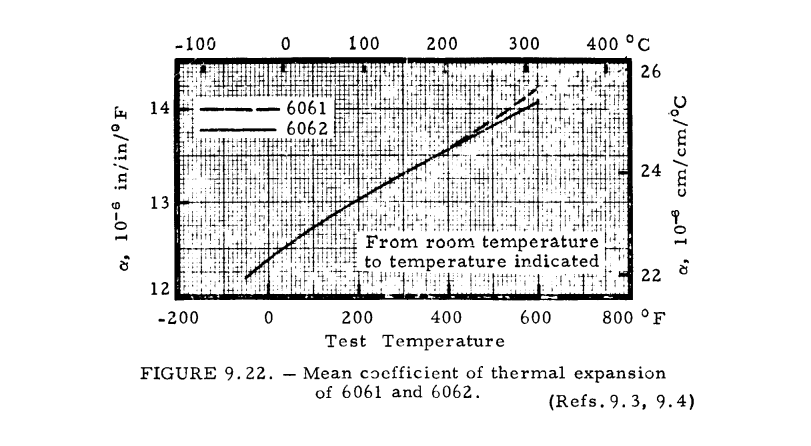
\includegraphics[width=0.8\textwidth]{Al_alpha_values}}
				\caption{Coefficient of thermal expansion of aluminum as a function of temperature}
				\label{fig:al_alpha}
			\end{figure}
			
			Though no numerical data was provided, the temperature-dependent aluminum CTE values can be approximated from this graph, shown in Table~\ref{tab:CTE_Al} in the Appendix.
			From this, we obtain the reference-temperature CTE (\specActuatorCTE) used in Chapter~\ref{chap:design},
			but the true value varies between \SI{21.8}{\micro\meter\per\meter\per\degreeCelsius} and \SI{23.5}{\micro\meter\per\meter\per\degreeCelsius} as $\Tcold \leq T \leq \Thot$.
			These introduce nonlinear behavior, resulting in quantifiable error.

		\subsection{Machine Tolerances}
		\label{subsec:sat:error:mach}

			General machine dimension tolerances depend on the capabilities of the manufacturing devices available.
			It is reasonable to assume that Sandia's tolerance capabilities meet or exceed those of standard Computer-Numerical Control (CNC) mills.
			The values represented in the engineering drawings (Appendix~\ref{app:drawings}) are taken from HAAS VF-2 series specifications \cite{haas_vf2_specs}.

			\begin{wrapfigure}{l}{.4\textwidth}
				\centering
				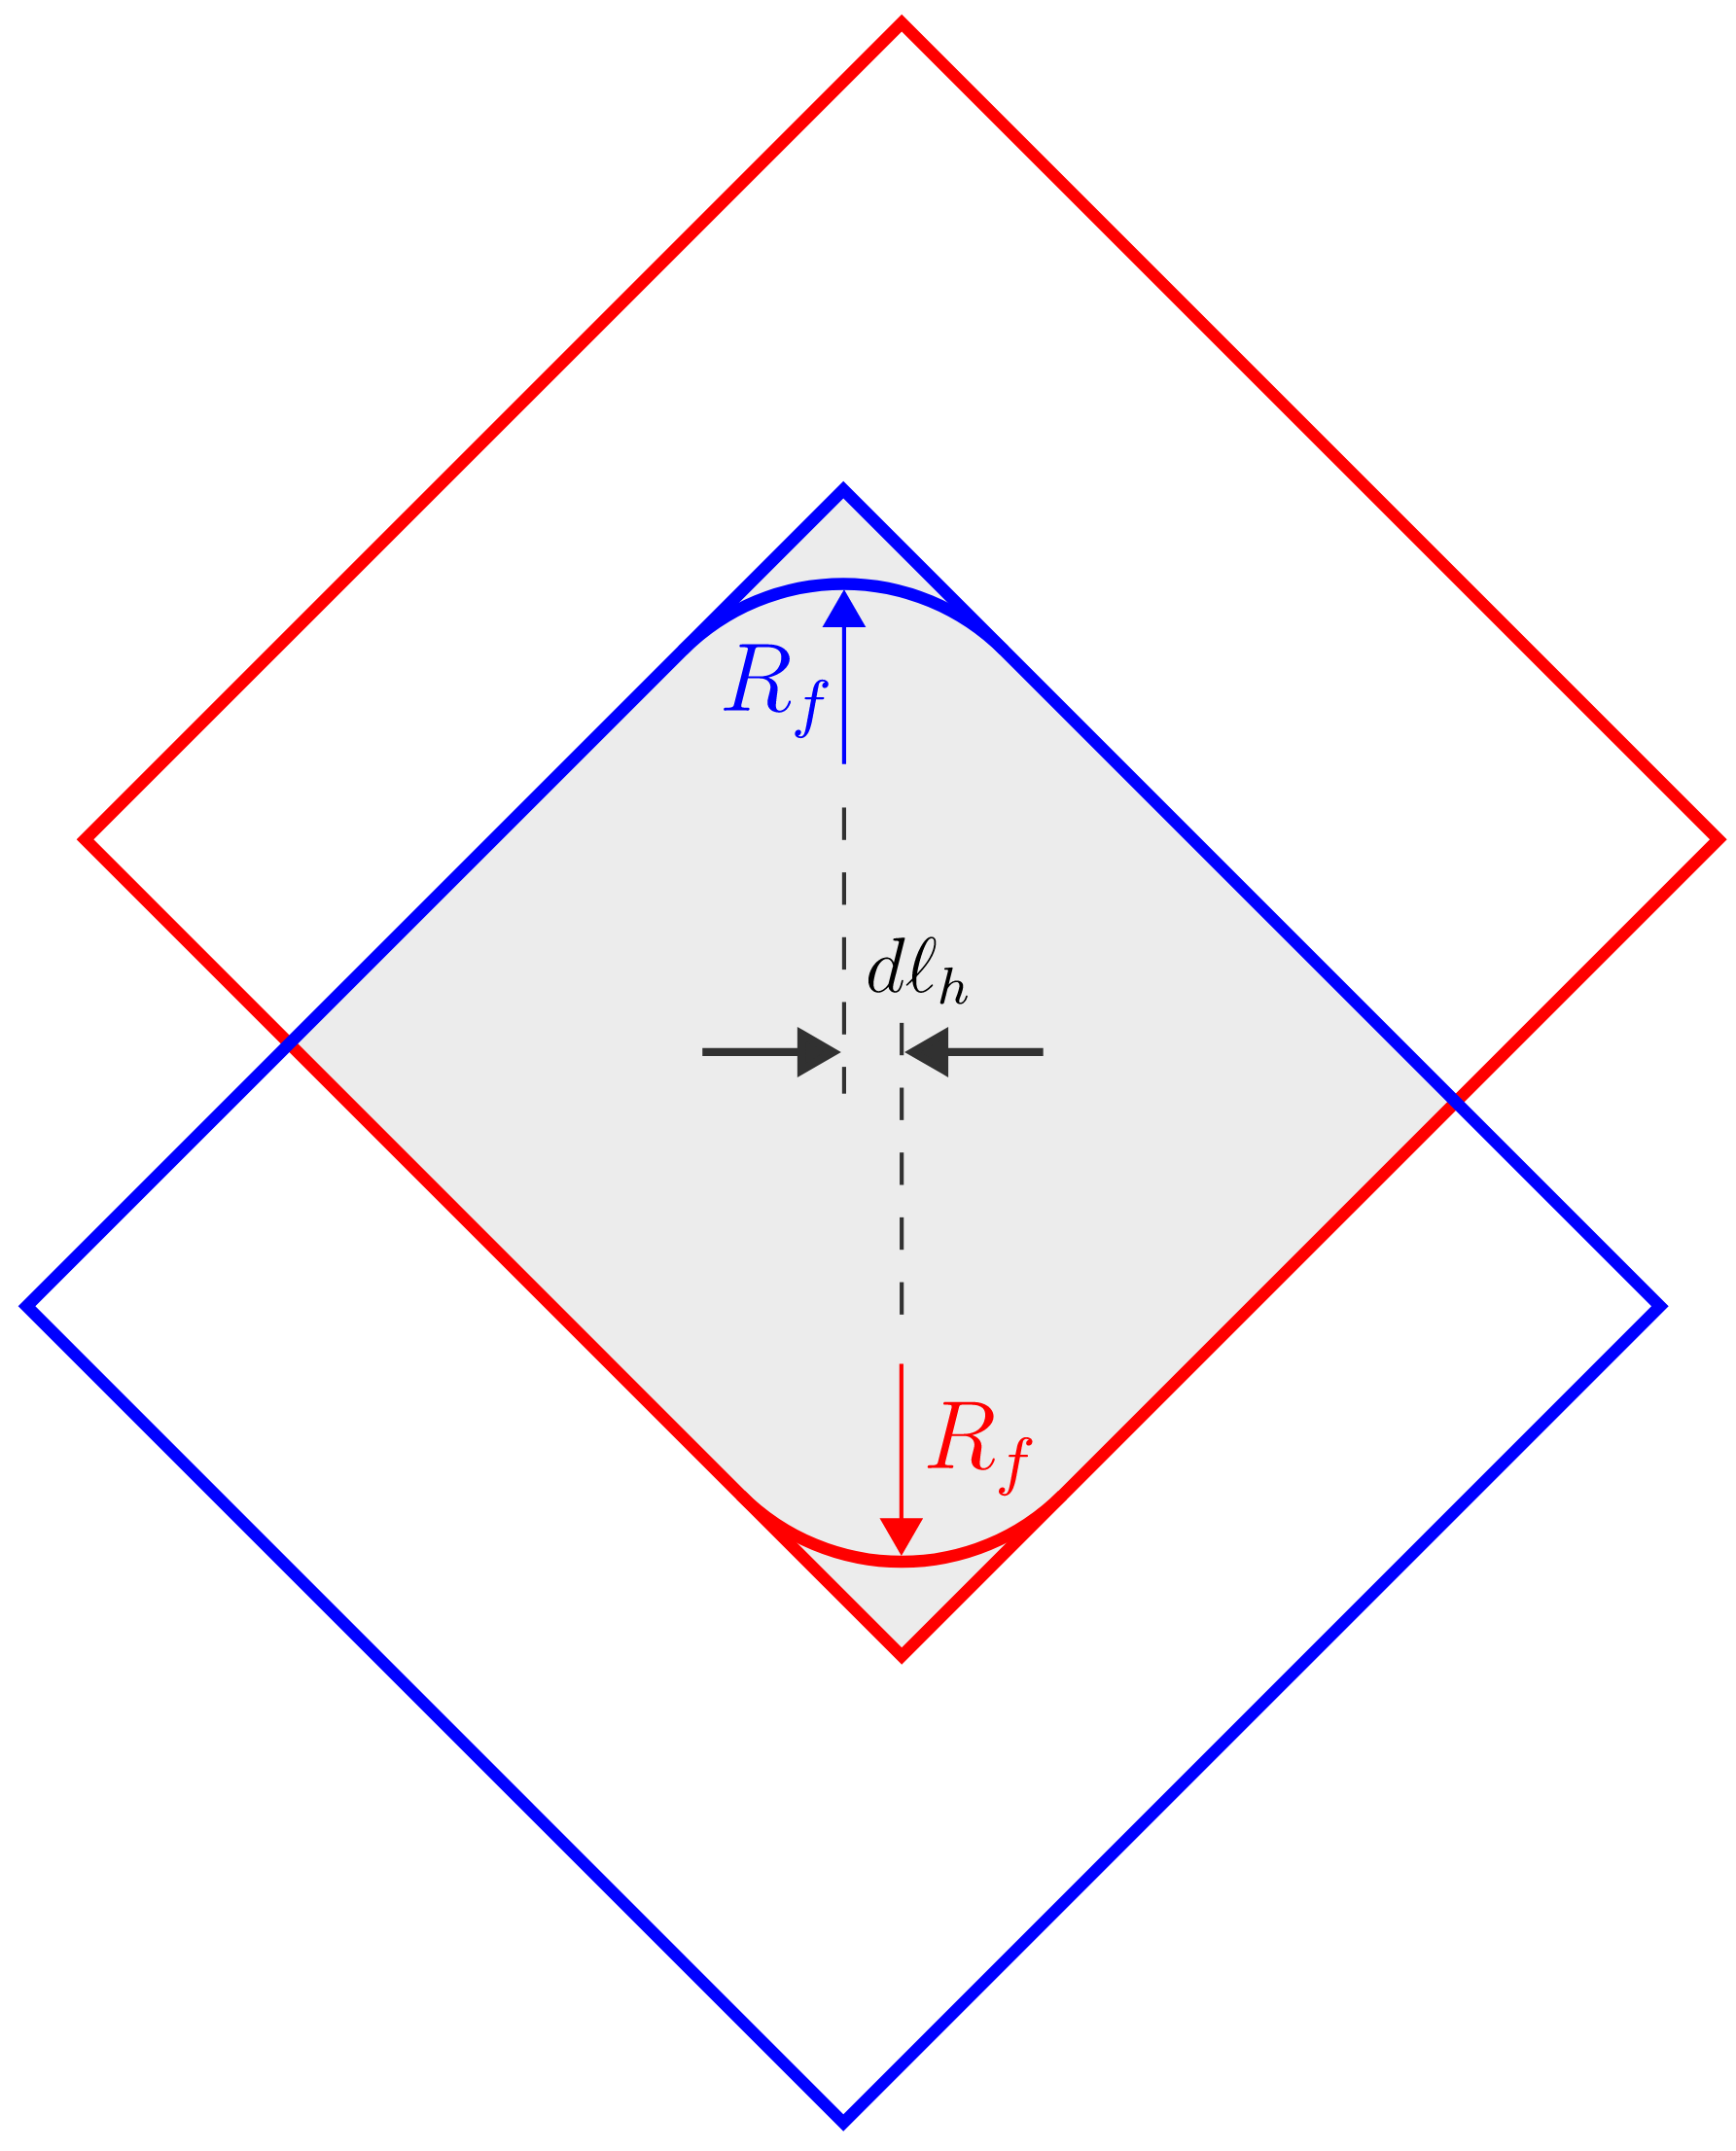
\includegraphics[width=.39\textwidth]{orif_error.png}
				\caption{Orifice error modes}
				\label{fig:orif_error}
			\end{wrapfigure}

			The two square holes that make the orifice will be machined with Sinker EDM. Two critical tolerances significantly influence the effective diameter of the orifice:
			the horizontal position of each hole and the fillet radii at the top and bottom vertices. The side vertices are made by the intersection of two straight cuts and can be assumed to be sharp.
			Figure~\ref{fig:orif_error} depicts these two error modes. Milco Wire EDM, Inc \todo{Update with Xometry quote once obtained} quoted the operation (attached in Appendix~\ref{app:datasheets}).
			They can achieve a minimum fillet radius $R_f = \SI{76.2}{\micro\meter}$ and horizontally position each orifice to a tolerance of \SI{12.7}{\micro\meter}.
			This horizontal error compounds if the leading orifice is machined too far left and the trailing orifice is machined too far right;
			the maximum error is twice this value. Thus, $d \ell_h = \SI{25.4}{\micro\meter}$.
			Vertical error can be more readily dealt with individually; thus, the noncompounding vertical error is defined as $d \ell_v = \SI{12.7}{\micro\meter}$.

		\subsection{Heat Transfer}
		\label{subsec:sat:error:dT}

			\todo{Thermal analysis from COMSOL to find final temperature of actuator and mount after 60s and at SS}

		\subsection{Bellows Spring Reactions}
		\label{subsec:sat:error:bellows}

			As the actuator deflects and drives the valve stem downwards or pulls it upwards, the two bellows act as springs and provide a slight reaction force, possibly compressing or stretching the valve stem and actuator.
			Since each part behaves as a spring, the resulting coupled spring assembly is complex and requires a comprehensive force balance analysis to reconcile the final deflections.

		Each of these sources of error impacts the entire system. Since the behavior of each subsystem is coupled, the effect of these errors on the final output of the \device\ can only be analyzed by a rigorous static system analysis.
		The transfer function derived in the following section provides a tool for analysis of deterministic and stochastic error propagation across the full temperature range.

	\section{Transfer Function Derivation}
	\label{app:calcs:TF}

		Derivation of the System Transfer Function in Section~\ref{sec:sat:TF} passed over certain calculations for brevity. They are given here.

		\subsection{Thermal Expansion}
		\label{app:calcs:TF:G_therm}

			Constants used in equations \eqref{eq:G_therm_1 -- eq:G_therm_last} are as follows.

			Material coefficients of thermal expansion:

			\begin{itemize}
				\item Aluminum (Al): \specActuatorCTE\cite[Table~9-22]{ref_NASA_specs_Al}
				\item Allvar (ALLV): \specMountCTE\cite{ref_AllvarAlloys}
				\item Invar 36 (Inv): \specInvarCTE\cite{ref_Carpenter_Inv}
				\item Inconel 718 (Inc): \specInconelCTE\cite{ref_SpecialMetals_Inc}
			\end{itemize}

			and the machined dimensions $\ell_{i_0}$ from Appendix~\ref{app:drawings}:

			\begin{itemize}
				\item $\ell_{M_0} = \SI{38.541}{\milli\meter} - \SI{0.55}{\milli\meter} = \SI{38.041}{\milli\meter}$\footnote{Top of the mount, for simplicity, is assumed to be the underside of the compressed belleville washer. Since this height is dependent on the use case, we will assume a \SI{0.05}{\milli\meter} compression.}
				\item $\ell_{A_0} = \SI{32.991}{\milli\meter}$
				\item $\ell_{S_0} = \SI{70.72}{\milli\meter} - \SI{32.86}{\milli\meter} = \SI{37.86}{\milli\meter}$
				\item $\ell_{T_0} = \SI{22.86}{\milli\meter}$
				\item $\ell_{B_0} = \ell_{T_0} = \SI{22.86}{\milli\meter}$
				\item $\ell_{V_0} = \SI{32.86}{\milli\meter} - \SI{27.86}{\milli\meter} = \SI{5}{\milli\meter}$
				\item $\ell_{H_0} = \SI{63.72}{\milli\meter}$
				\item $\ell_{W_0} = \SI{10}{\milli\meter}$
			\end{itemize}

		\subsection{Force Balance}
		\label{app:calcs:TF:force_balance}

			The spring-assembly model of the \device, introcuded in Section~\ref{subsec:sat:TF:force_balance}, is shown again in Figure~\ref{fig:app_springs}.

			\begin{figure}[H]
				\centering
				\begin{minipage}{.45\textwidth}
					\centering
					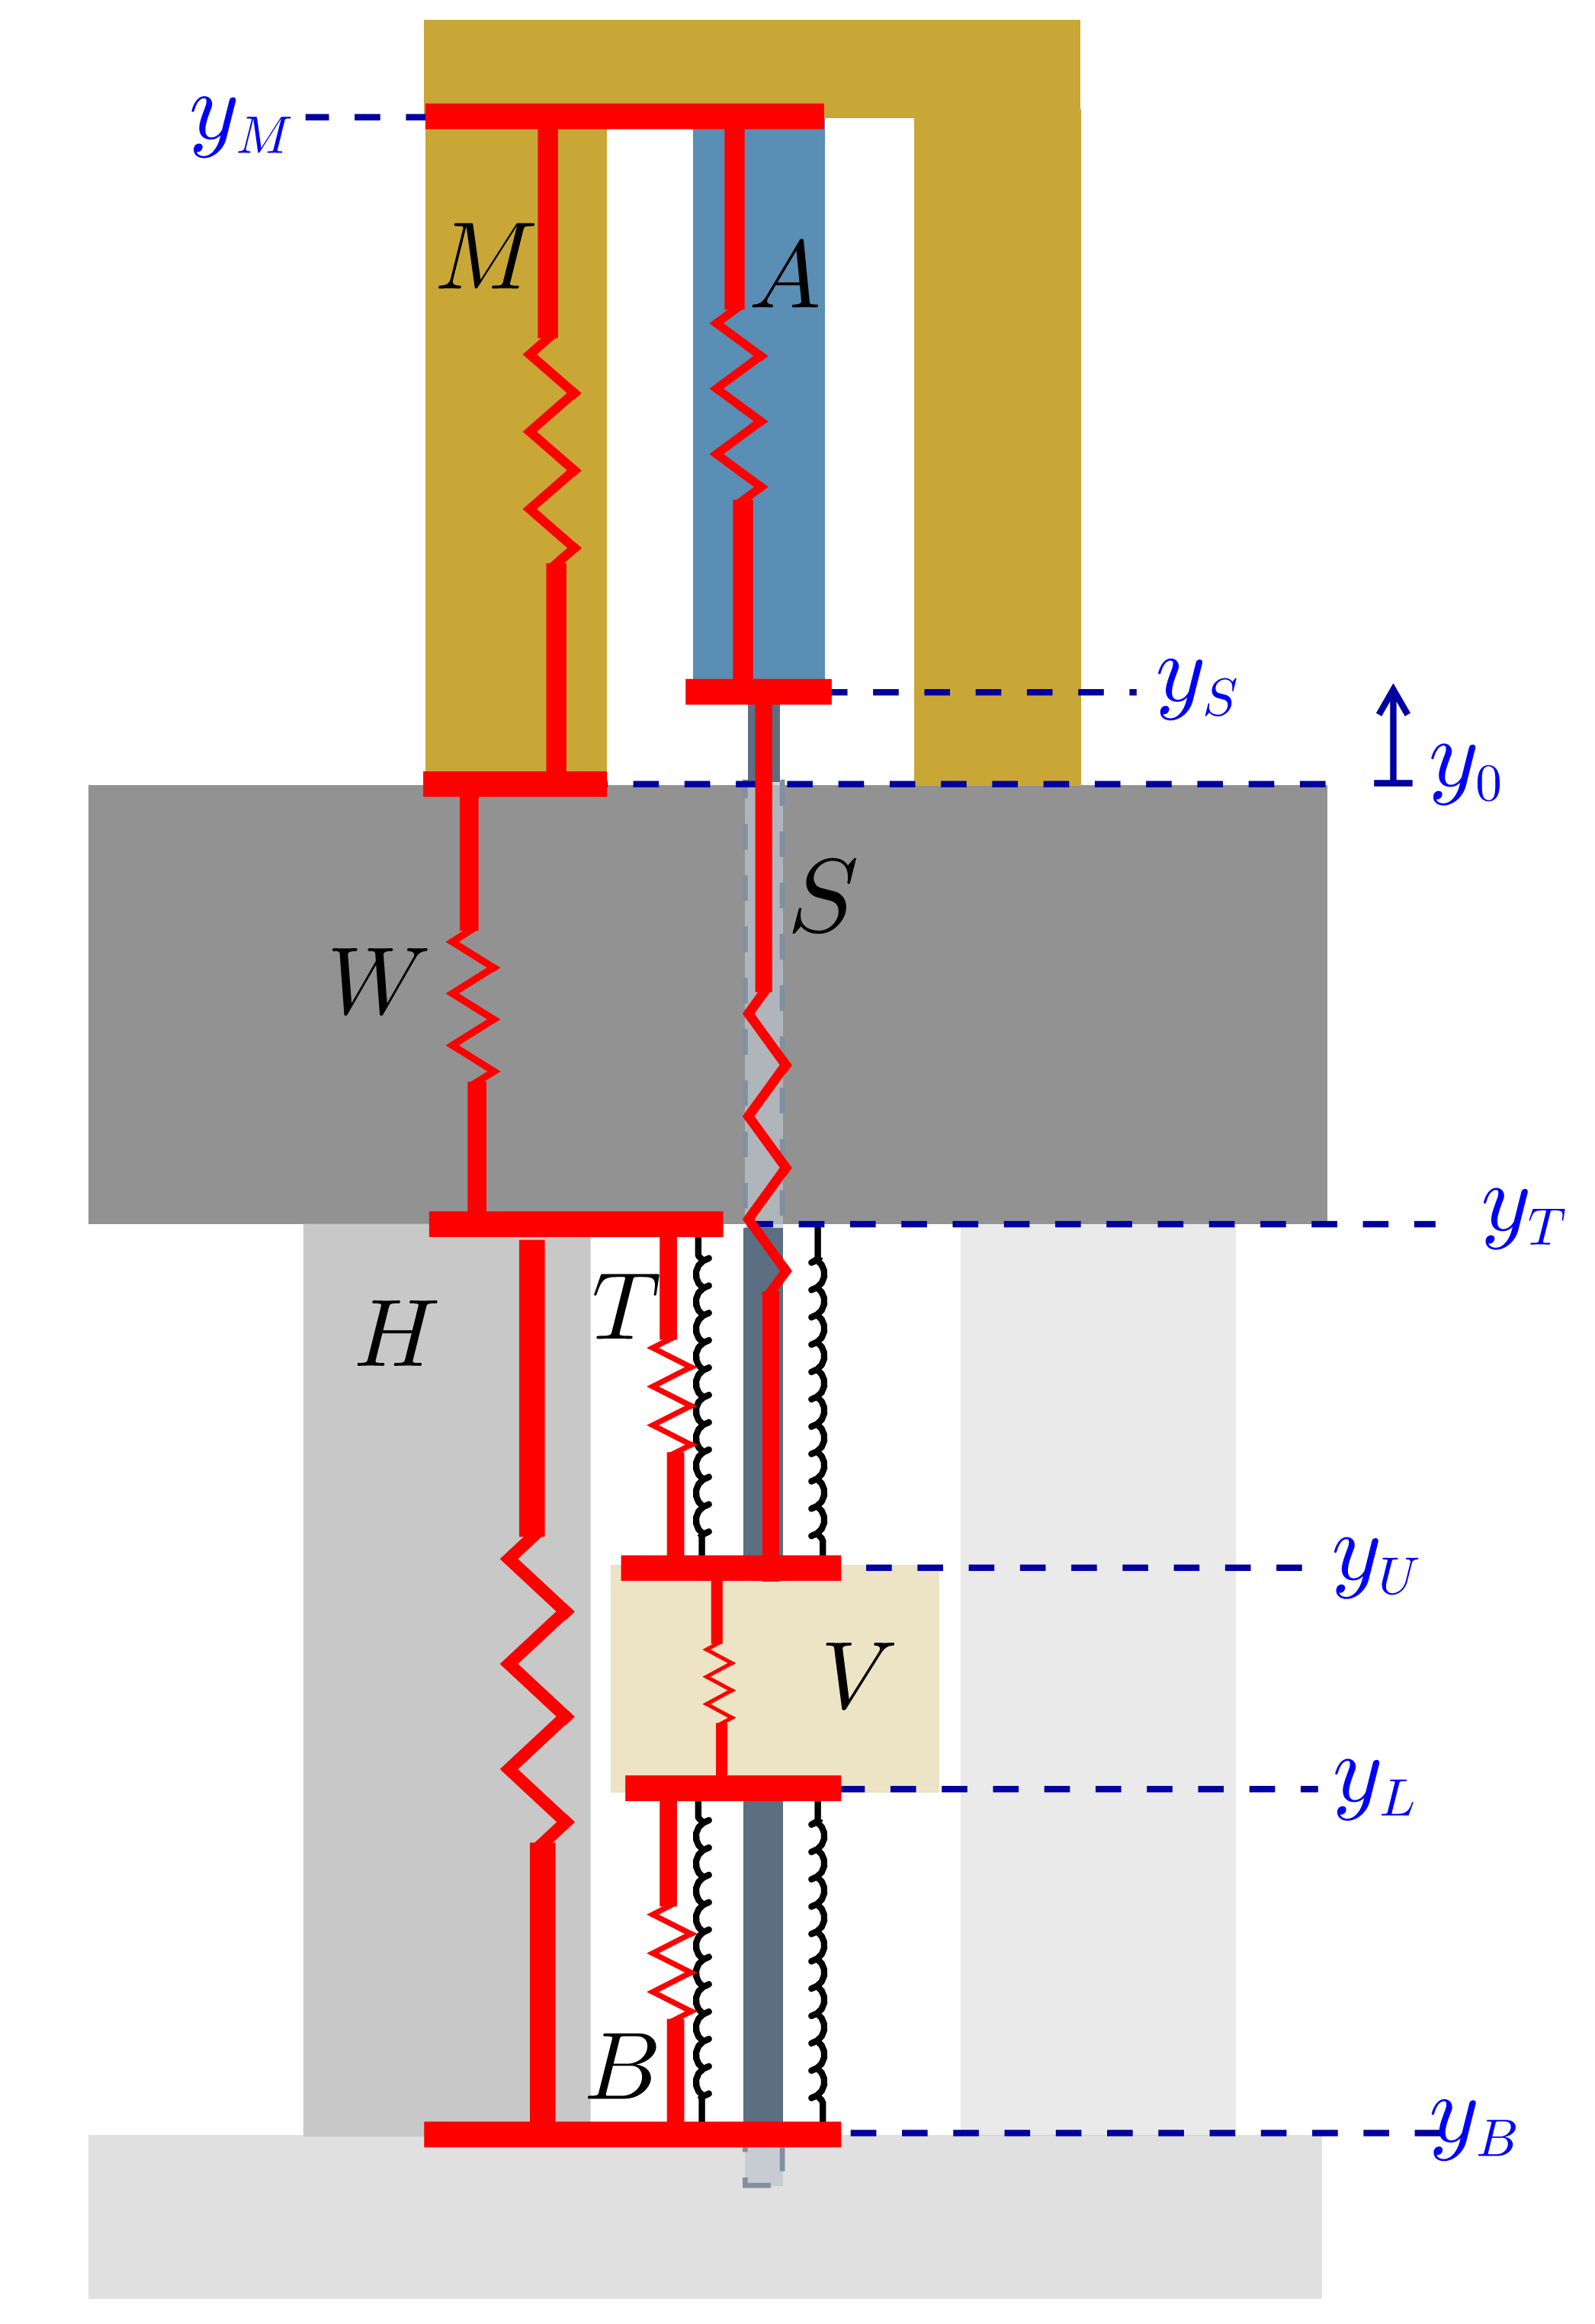
\includegraphics[height=.5\textheight]{springs.png}
					\subcaption{\device\ spring mechanism}
					\label{fig:app_springs_full}
				\end{minipage}
				\hfill
				\begin{minipage}{.45\textwidth}
					\centering
					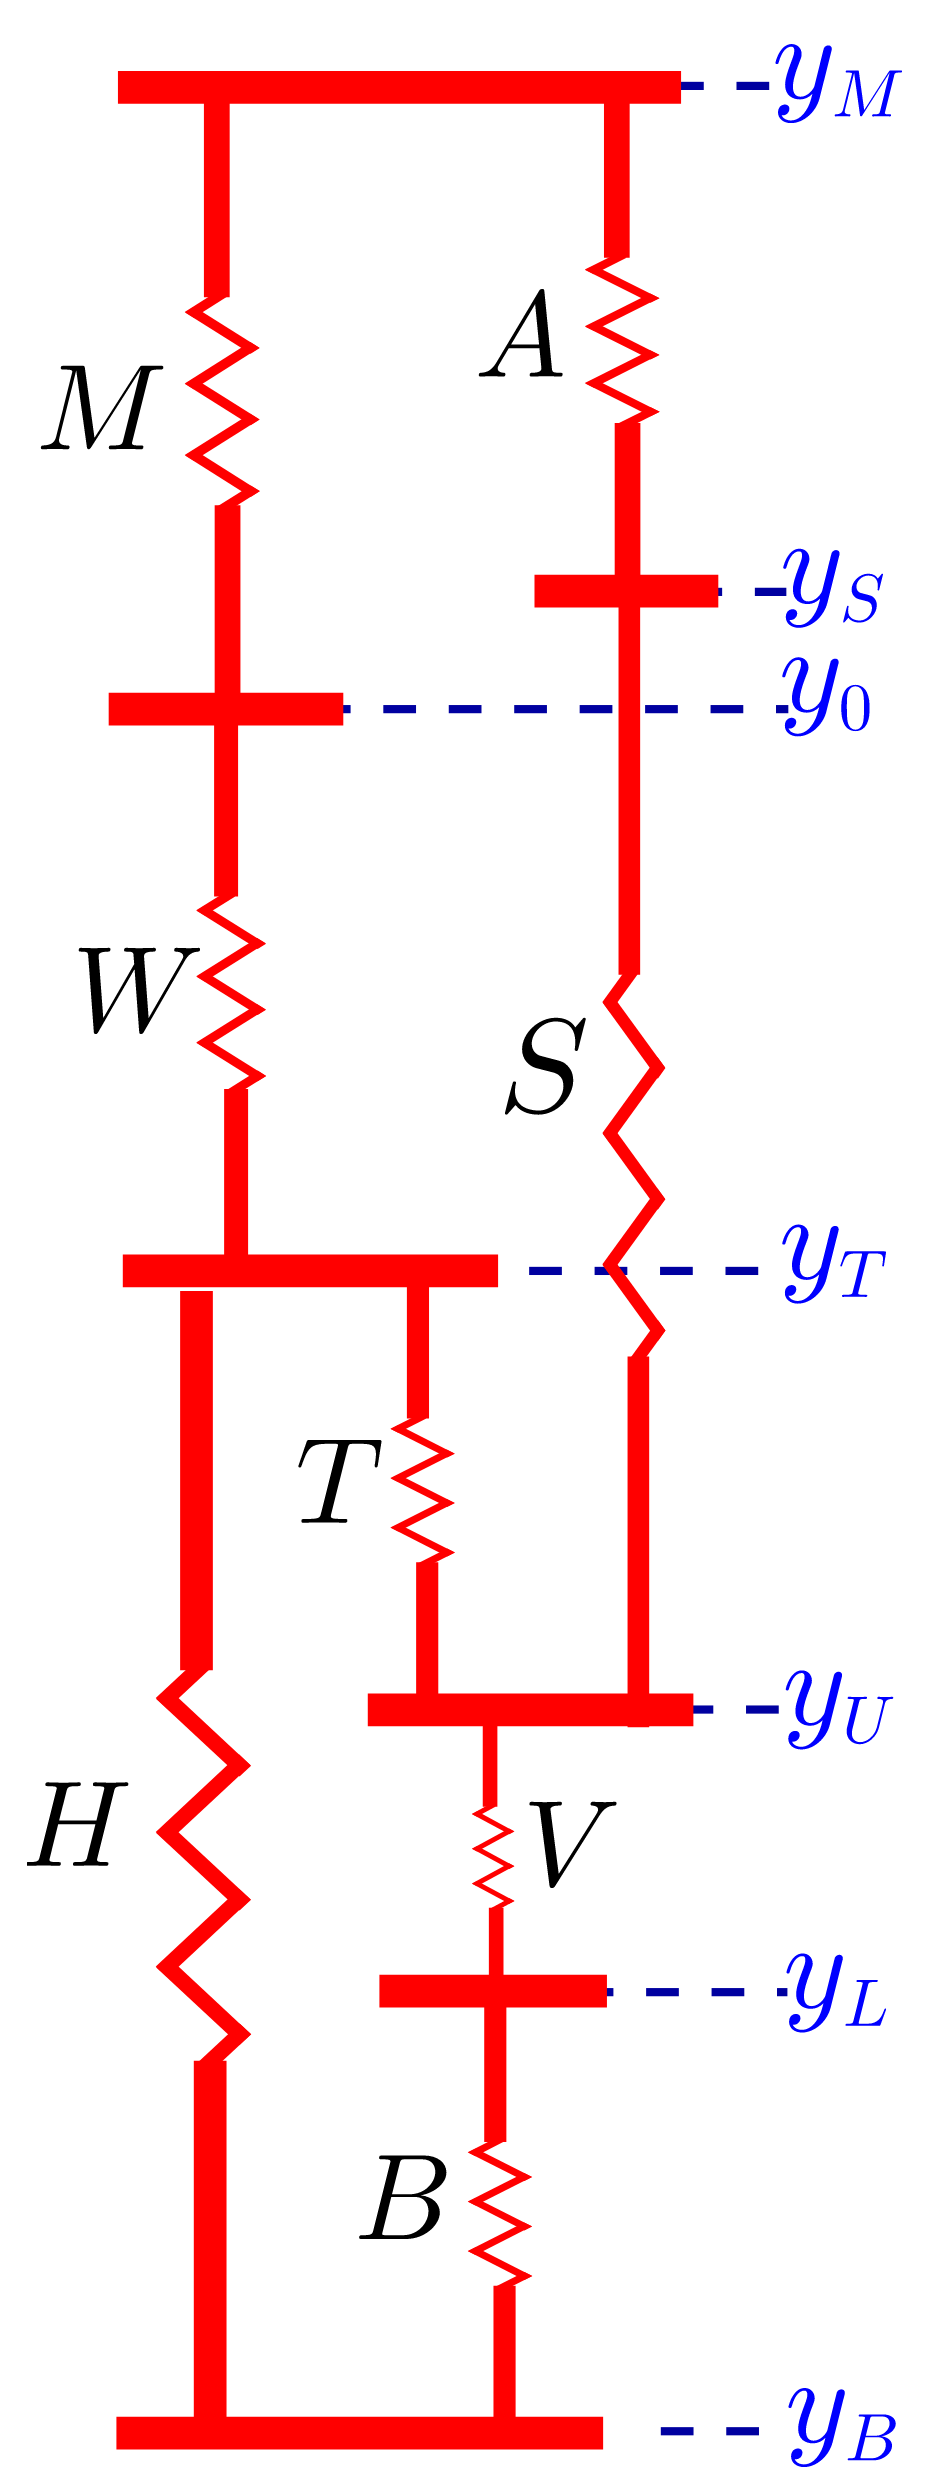
\includegraphics[height=.5\textheight]{springs_simp.png}
					\subcaption{\device\ spring mechanism, simplified}
					\label{fig:app_springs_simp}
				\end{minipage}
				\caption{Spring deflection}
				\label{fig:app_springs}
			\end{figure}

			Solution of the final lengths of these springs requires a system of equations, derived using static force analysis.
			We will use Figure~\ref{fig:springs_simp}, which accurately depicts the contact between parts, as our guide.
			The system contains seven nodes, labeled according to their subscripted position $y$, that we will use as the basis for our equations.
			For each nodal force balance, let us assume that the springs act along one degree of freedom (DOF), inducing no rotational moment.
			This is a safe assumption because, although the springs are depicted as spaced apart horizontally, they are concentric in the actual design.

			Equating upper and lower vertical forces at each node produces the following system of equations:

			\newcommand{\circlab}[1]{%
				\tikz[baseline=(char.base)]{
					\node[shape=circle, draw, inner sep=1pt,
						minimum size=1.5em] (char) {$#1$};
				}%
			}

			\newcommand{\ellipselab}[1]{%
				\tikz[baseline=(char.base)]{
					\node[shape=ellipse, draw, inner sep=1pt,
						minimum width=3.2em, minimum height=1.6em] (char) {$#1$};
				}%
			}

			\begin{equation}
				\left\{
				\begin{array}{ll}
					\circlab{y_M} & F_M + F_A = 0 \\[6pt]
					\circlab{y_S} & F_A = F_S \\[6pt]
					\circlab{y_0} & F_M = F_W \\[6pt]
					\circlab{y_T} & F_W = F_H + F_T \\[6pt]
					\circlab{y_U} & F_V = F_T + F_S \\[6pt]
					\circlab{y_L} & F_V = F_B \\[6pt]
					\circlab{y_B} & F_H + F_B = 0 \\
				\end{array}
				\right.
			\end{equation}

			This produces seven equations for eight unknown forces $(F_M, F_A, F_S, F_T, F_B, F_V, F_H, \text{ and } F_W)$.
			One might observe that this system remains indeterminate without one additional equation\footnote{It is well-established in the field of Linear Algebra that a system of linear equations with more equations than unknowns is linearly dependent (one or more equations is redundant) or self-contradictory, while that with more unknowns than equations is incomplete. A determinate system of equations requires exactly as many linearly independent equations as unknowns\cite{ref_Anton}.}.
			In fact, this system is linearly dependent and, when rearranged, contains a pair of redundant equations.

			From equations $y_M$, $y_S$, and $y_0$:

			\begin{align*}
				F_M &= F_W \\
				F_A &= -F_M = -F_W \\
				F_S &= F_A = -F_W
			\end{align*}

			From equations $y_L$ and $y_B$:

			\begin{align*}
				F_B &= F_V \\
				F_H &= -F_B = -F_V
			\end{align*}

			Substituting these into equations $y_T$ and $y_U$:

			\begin{align*}
				F_W &= -F_V + F_T \\
				F_V &= F_T - F_W
			\end{align*}

			These equations are linearly dependent and therefore redundant; one can easily rearrange one to equal the other. Thus, we will strike equation~$y_U$, leaving us six equations and eight unknowns.

			By Hooke's Law\cite{ref_Young_Freedman}, $F = k \Delta X$, we can substitute their forces for known spring constants, known undeformed lengths (as output by the thermal transfer functions), and unknown final lengths.
			The final two equations are supplied by two parallel length equalities: between $y_M$ and $y_U$ and between $y_T$ and $y_B$.

			\begin{equation}
				\left\{
				\begin{array}{ll}
					\circlab{y_M} & k_M(L_M - \ell_M) + k_A(L_A - \ell_A) = 0 \\[6pt]
					\circlab{y_S} & k_A(L_A - \ell_A) = k_S(L_S - \ell_S) \\[6pt]
					\circlab{y_0} & k_M(L_M - \ell_M) = k_W(L_W - \ell_W) \\[6pt]
					\circlab{y_T} & k_W(L_W - \ell_W) = k_H(L_H - \ell_H) + k_T(L_T - \ell_T) \\[6pt]
					\circlab{y_L} & k_V(L_V - \ell_V) = k_B(L_B - \ell_B) \\[6pt]
					\circlab{y_B} & k_H(L_H - \ell_H) + k_B(L_B - \ell_B) = 0 \\[6pt]
					\ellipselab{y_M \rightarrow y_U} & L_M + L_W + L_T = L_A + L_S \\[6pt]
					\ellipselab{y_T \rightarrow y_B} & L_H = L_T + L_V + L_B
				\end{array}
				\right.
			\end{equation}

			Now we have a system of eight equations with eight unknowns. These can be analytically solved using a matrix calculator by rearranging as follows:

			\begin{equation}
				\left\{
				\begin{array}{l}
					k_M L_M + k_A L_A = k_M \ell_M + k_A \ell_A \\[6pt]
					k_A L_A - k_S L_S = k_A \ell_A - k_S \ell_S \\[6pt]
					k_M L_M - k_W L_W = k_M \ell_M - k_W \ell_W \\[6pt]
					k_W L_W - k_T L_T - k_H L_H = k_W \ell_W - k_T \ell_T - k_H \ell_H \\[6pt]
					k_V L_V - k_B L_B = k_V \ell_V - k_B \ell_B \\[6pt]
					k_B L_B + k_H L_H = k_B \ell_B + k_H \ell_H \\[6pt]
					L_M - L_A - L_S + L_T + L_W = 0 \\[6pt]
					L_T + L_B + L_V - L_H = 0
				\end{array}
				\right.
			\end{equation}

			\begin{equation}
				\forceMatrix
			\label{eq:app_matrix}
			\end{equation}

			Each undeformed length $\ell$ is provided by the thermal transfer functions. With the exception of the two bellows, whose spring constants are given, each spring constant $k$ is calculated by material properties and part geometry\cite[Eq.~4-2]{ref_Hibbeler}:
			
			\begin{equation}
				k = \frac{EA}{\ell}
			\end{equation}
			
			where $E$ is the elastic modulus, $A$ is the cross-sectional area, and $\ell$ is defined as before. Below are the values required to find the spring constant of each part.
			
			\subsubsection{Mount}
			\label{app:calcs:TF:force_balance:M}

				$E_M = E_{\text{ALLVAR}} = \specEALLV$\cite{ref_AllvarAlloys}
				
				$A_M = \frac{\pi}{4} (OD^2 - ID^2) = \frac{\pi}{4} [(\SI{25}{\milli\meter})^2 - (\SI{18}{\milli\meter})^2] = \SI{236.4}{\milli\meter\squared}$

			\subsubsection{Actuator}
			\label{app:calcs:TF:force_balance:A}

				$E_A = E_{\text{Aluminum}} = \specEAl$\cite[p.~39]{ref_NASA_specs_Al}

				$A_A = \frac{\pi}{4} D^2 = \frac{\pi}{4} (\SI{18}{\milli\meter})^2 = \SI{254.5}{\milli\meter\squared}$

			\subsubsection{Valve Stem}
			\label{app:calcs:TF:force_balance:S}

				$E_S = E_{\text{Invar}} = \specEInv $\cite{ref_Carpenter_Inv}

				$A_S = \frac{\pi}{4} D^2 = \frac{\pi}{4} (\SI{3.353}{\milli\meter})^2 = \SI{2.6}{\milli\meter\squared}$
				
			\subsubsection{Bellows}
			\label{app:calcs:TF:force_balance:TB}

				$k_T = \specBellowsK $\cite{ref_miniflex_design}

			\subsubsection{Valve Orifice}    
			\label{app:calcs:TF:force_balance:V}
			
			$E_V = E_{\text{Invar}} = \specEInv $
			
			$A_V = LW = (\SI{7}{\milli\meter}) (\SI{7}{\milli\meter}) = \SI{49}{\milli\meter\squared}$
			
			\subsubsection{Housing}    
			\label{app:calcs:TF:force_balance:H}

				$E_H = E_{\text{Invar}} = \specEInv $

				$A_H = LW = (\SI{72}{\milli\meter}) (\SI{40}{\milli\meter}) = \SI{2880}{\milli\meter\squared}$

			\subsubsection{Top wall}
			\label{app:calcs:TF:force_balance:W}

				$E_W = E_{\text{Invar}} = \specEInv $

				$A_W = A_H = \SI{2880}{\milli\meter\squared}$

			These spring constants are input into equation~\eqref{eq:app_matrix} to solve for the deformed length of each part.

		\subsection{Orifice Coefficients}
		\label{app:calcs:TF:K}

			Equations \eqref{eq:yF} and \eqref{eq:yR} provide the final position of the lower and upper orifice vertices, restated here:

			\begin{align}
				y_F &= L_M - L_A - L_S - K_V L_V \\
				y_R &= - K_H (2 L_W + L_H) 
			\end{align}

			The scaling constant $K_V$ defines the position of the upper vertex of the leading orifice, and $K_H$ the lower vertex of the trailing orifice, determined by its machined dimensions as shown in Figure~\ref{fig:K_pos}.

			\begin{wrapfigure}{l}{0.5\textwidth}
				\centering
				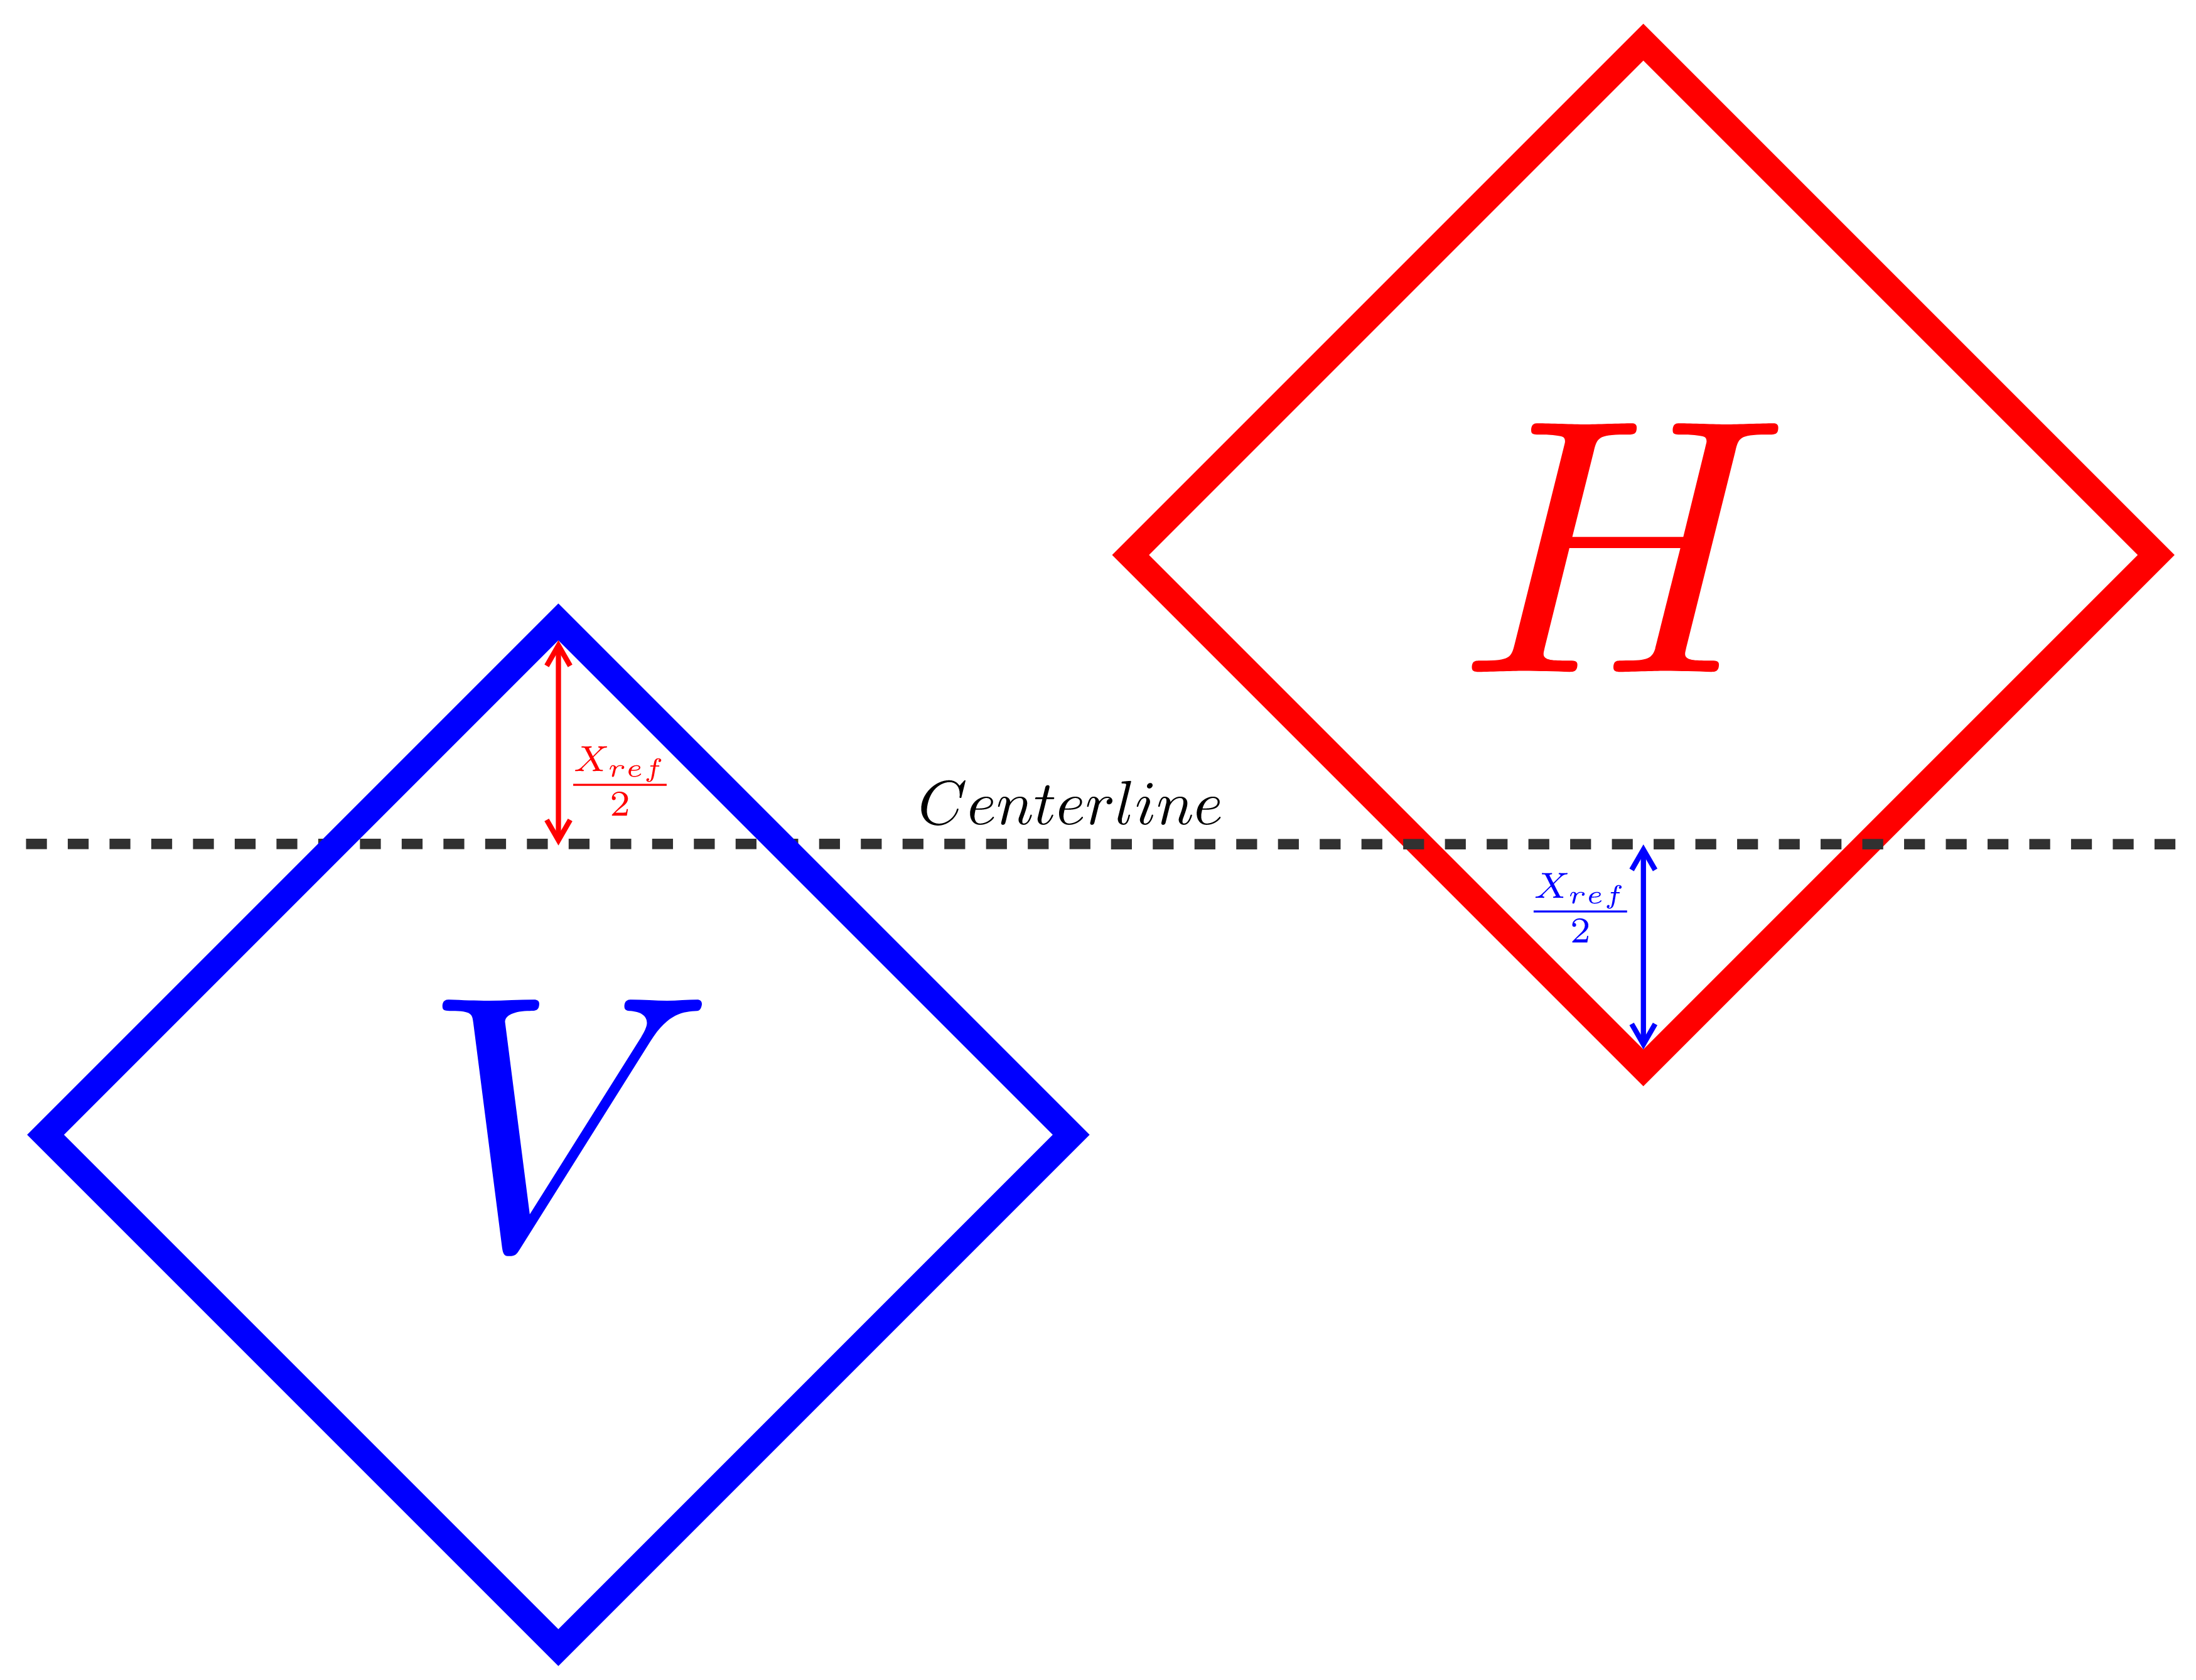
\includegraphics[width=0.48\textwidth]{K_pos.png}
				\caption{Orifice geometry}
				\label{fig:K_pos}
			\end{wrapfigure}

			As manufactured, $K_V \ell_{V_0}$ is defined as the distance from the top surface of the Valve Orifice $(y_T)$, whose machined height equals $\ell_{V_0}$, such that

			\begin{equation}
				K_V \ell_{v_0} = \frac{l_{v_0}}{2} - \left[ \frac{X_{ref}}{2} + d_{V_v} \right]
			\end{equation}

			where $d_{V_v}$ is the vertical position error of the EDM operation (defined as positive in the upwards direction), identical to the horizontal position error.

			Likewise, $K_H (2 \ell_{W_0} + \ell_{H_0})$ is defined as the distance from the top surface of the Housing Outlet $(y_0)$, whose machined height equals $(2 \ell_{W_0} + \ell_{H_0})$, such that

			\begin{equation}
				K_H (2 \ell_{W_0} + \ell_{H_0}) = \frac{(2 \ell_{W_0} + \ell_{H_0})}{2} + \left[ \frac{X_{ref}}{2} - d_{V_v} \right]
			\end{equation}

			therefore

			\begin{align}
				K_V &= \frac{1}{2} - \frac{\frac{X_{ref}}{2} + d \ell_{V_v}}{\ell_{V_0}} \\[6pt]
				K_H &= \frac{1}{2} + \frac{\frac{X_{ref}}{2} - d \ell_{H_v}}{2 \ell_{W_0} + \ell_{H_0}}
			\end{align}

			Note that the machined-length values are exact values as the position of the EDM cut is independent of any dimensional error in the valve orifice or housing outlet.

		\subsection{Orifice Machining Errors}
		\label{app:calcs:TF:dA}

			The error introduced directly into the area calculation in Section \ref{subsec:sat:error:mach} and \ref{subsubsec:sat:TF:orif:G_A} depends on the fillet radius $R_f$ and horizontal position error $d \ell_h$.

			Each fillet radius $R_f$ subtracts the following area from the orifice, depicted in Figure~\ref{fig:Rf}:

			\begin{equation}
				dA = (\textit{Orange area}) = (\textit{Square area}) - (\textit{Gray quarter circle}) = R_f^2 - \frac{1}{4} \pi R_f^2 = \frac{1}{4} (4 - \pi) R_f^2
			\end{equation}

			\begin{figure}[H]
				\centering
				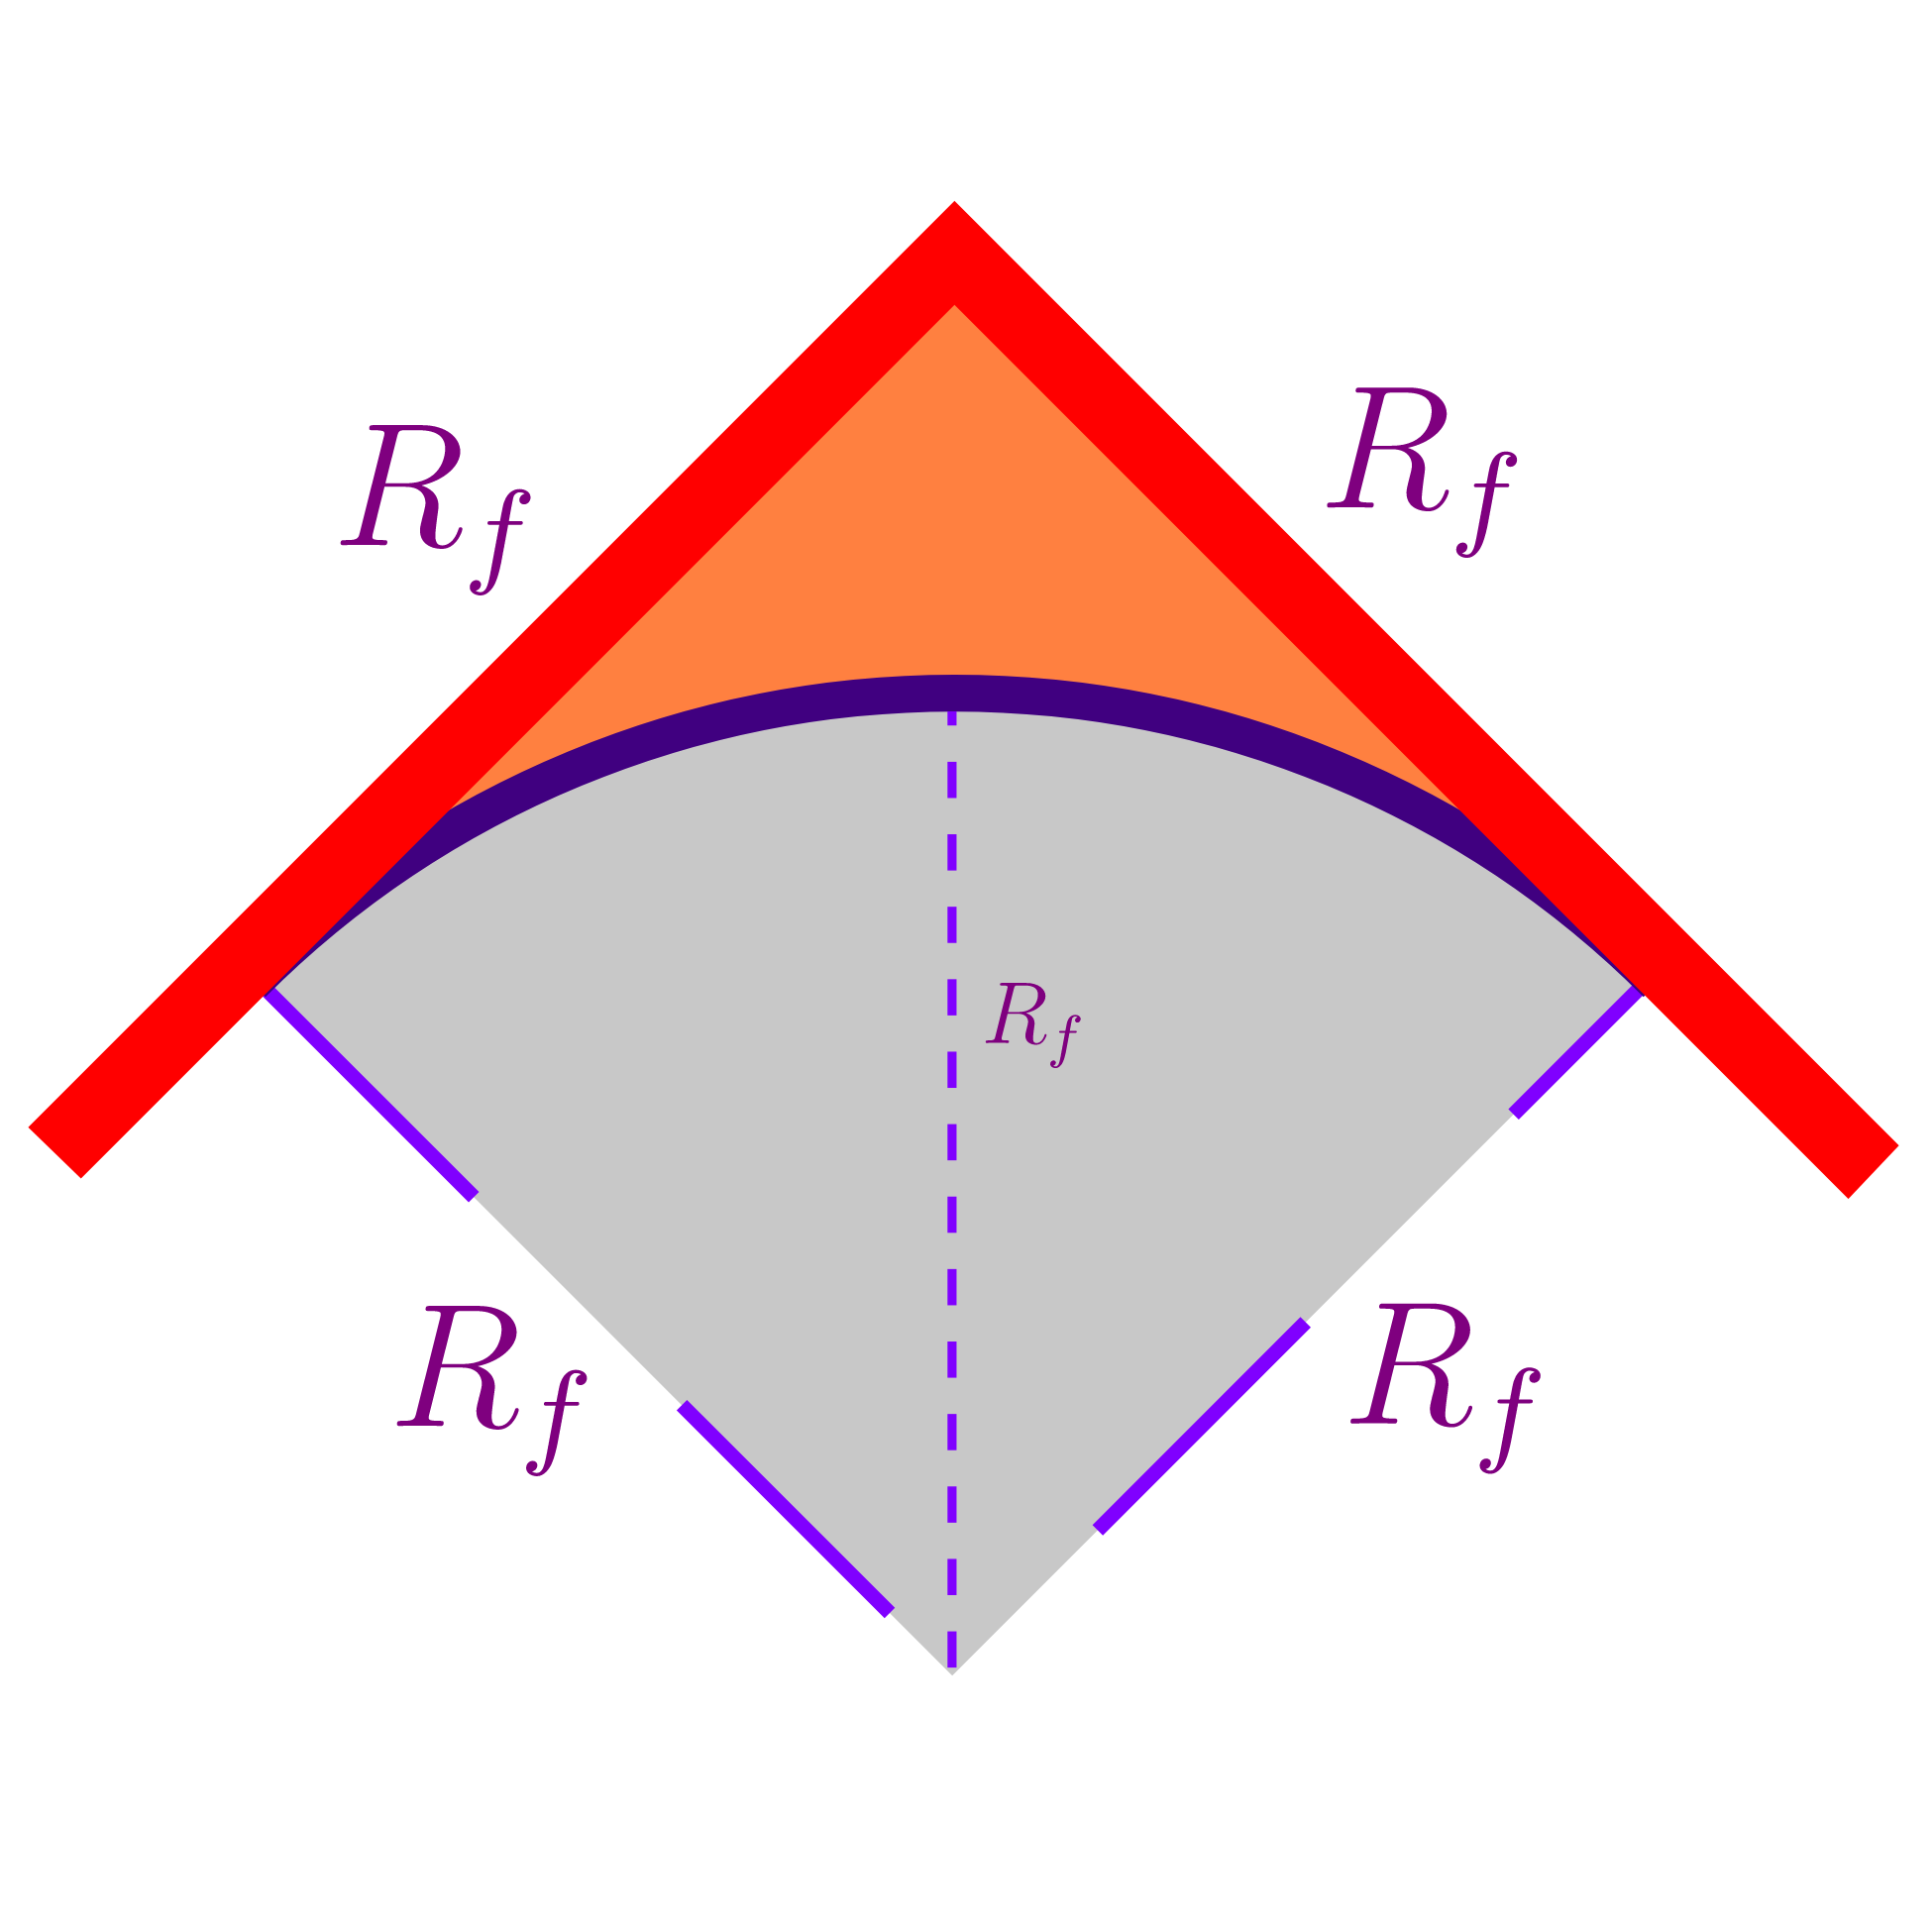
\includegraphics[width=.3\textwidth]{Rf.png}
				\caption{Fillet Radius Dimensions}
				\label{fig:Rf}
			\end{figure}

			Horizontal shift $d \ell_h$ changes the area as shown in Figure~\ref{fig:dl_h}, adding the green area and subtracting the orange.
			Ignoring the fillet radii, this results in the new area

			\begin{equation}
				A = (s + \frac{d \ell}{2}) (s - \frac{d \ell}{2}) = s^2 - \frac{d \ell^2}{2}
			\end{equation}

			\begin{figure}[H]
				\centering
				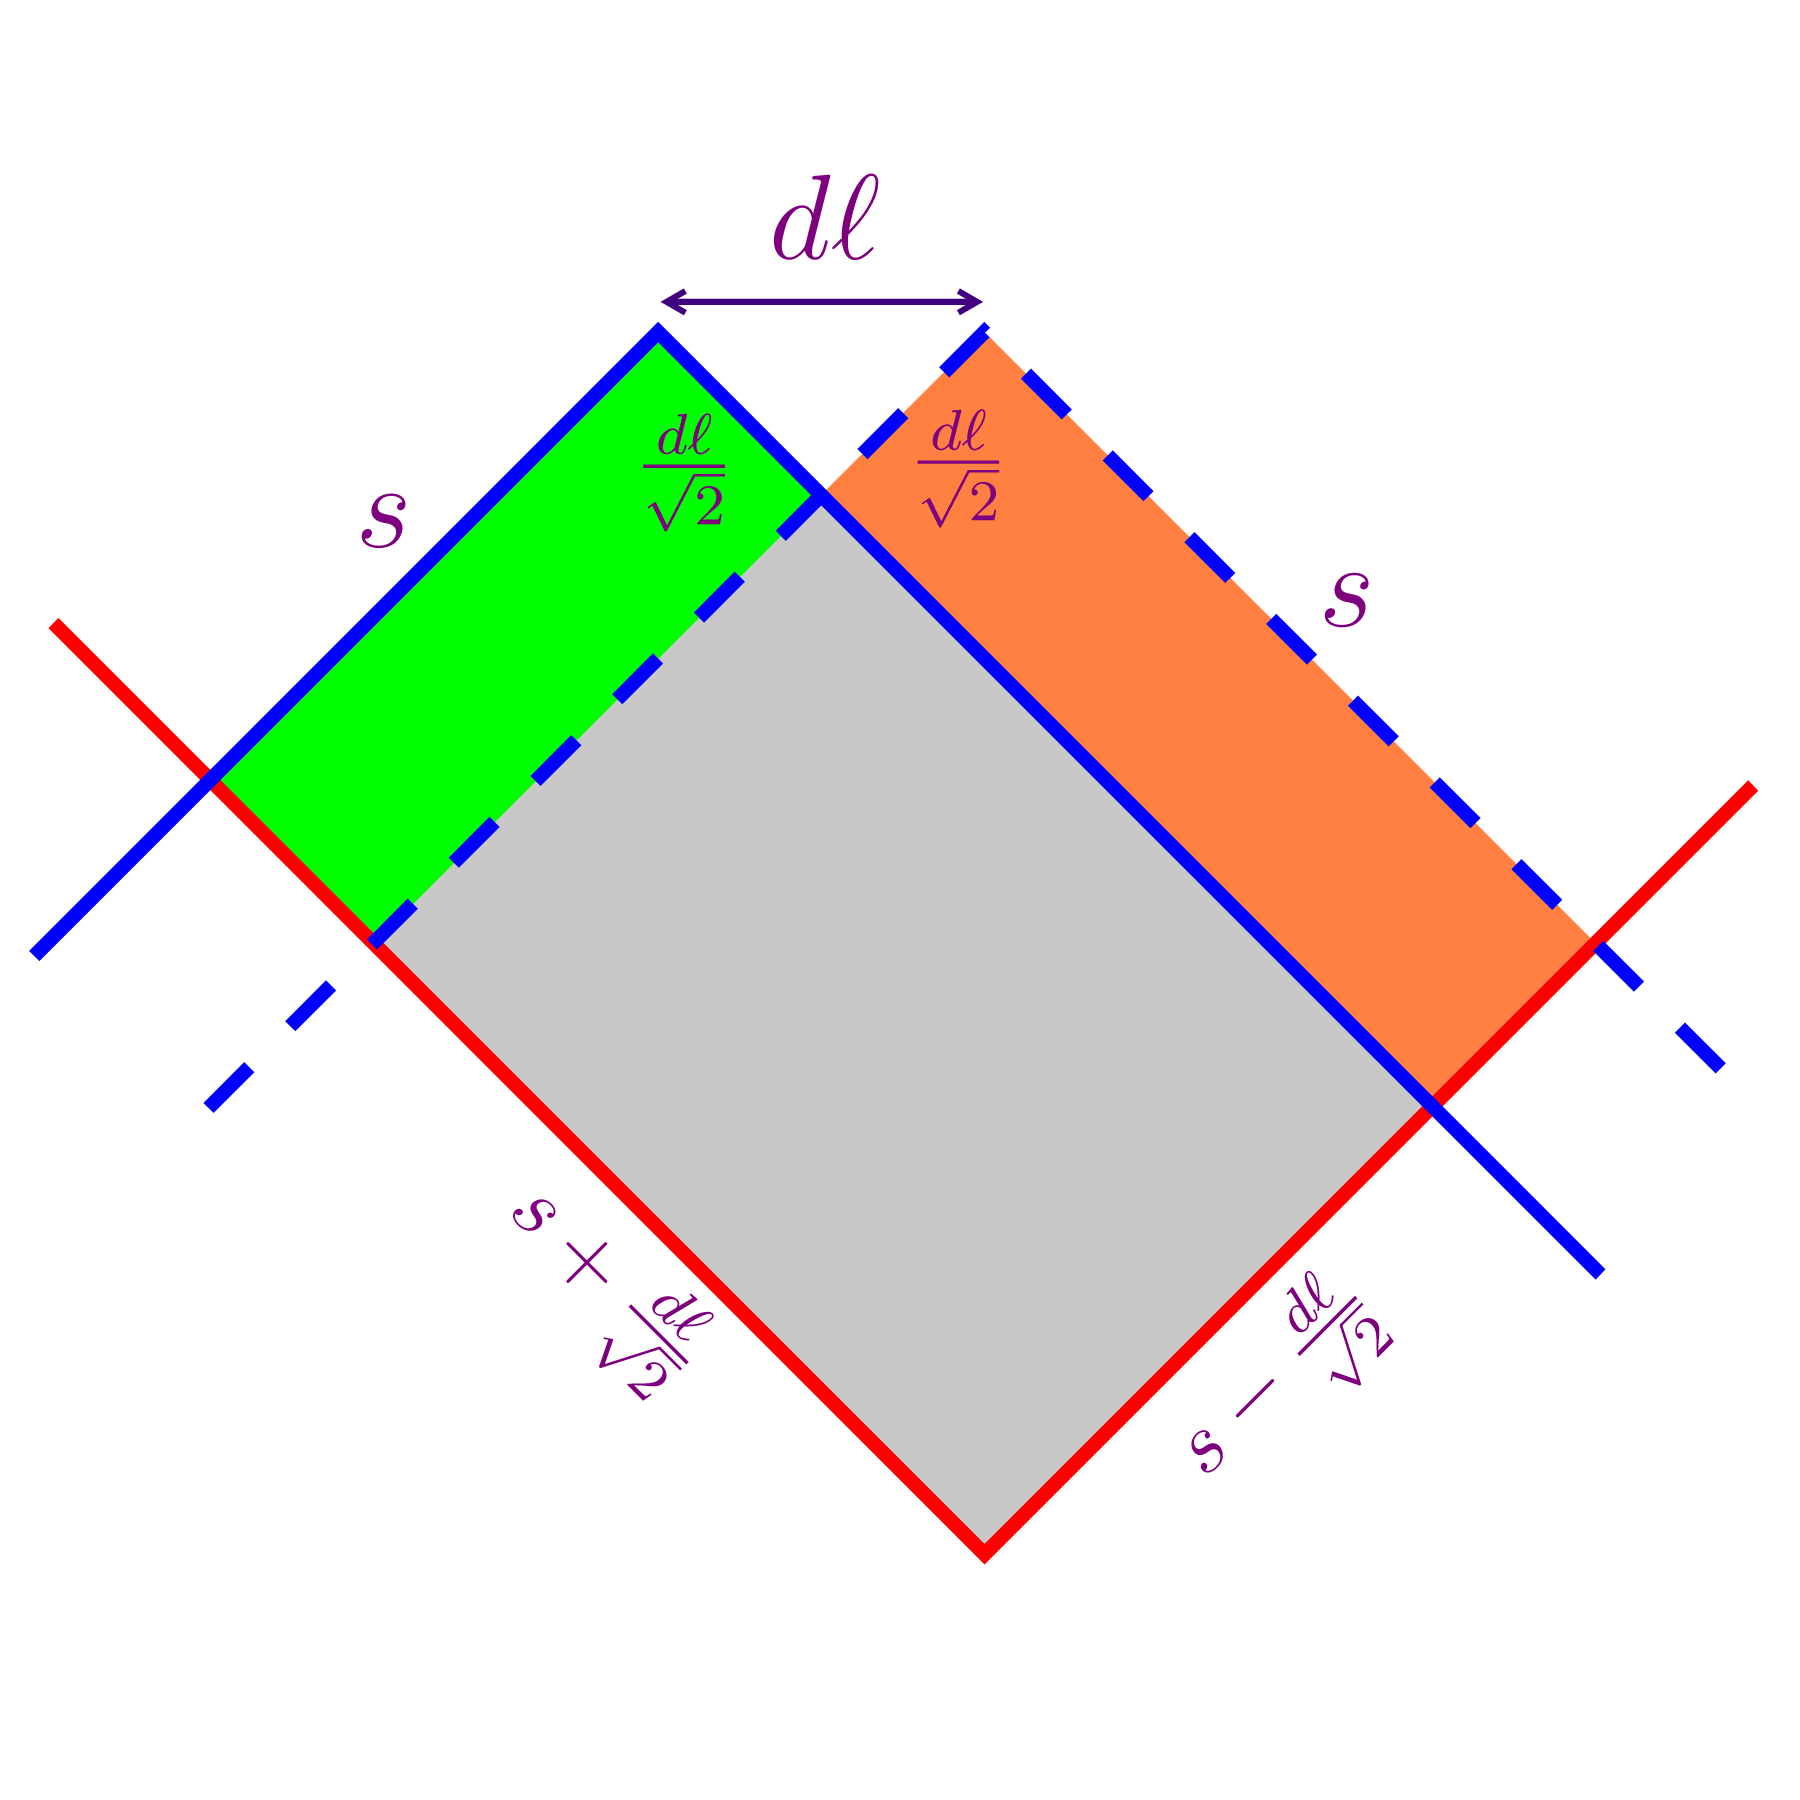
\includegraphics[width=.3\textwidth]{dl_h.png}
				\caption{Horizontal Offset Dimensions}
				\label{fig:dl_h}
			\end{figure}

			yielding the final orifice area as reflected in equation~\eqref{eq:GA}:

			\begin{equation}
				A = s^2 - \frac{1}{2} \left[ (4 - \pi) R_f^2 - d \ell^2 \right]
			\end{equation}

		\subsection{Function Output}
		\label{app:calcs:TF:results}

			Figure~\ref{fig:TF_res} demonstrates the ouput of the System Transfer Function given two worst-case combinations of the stochastic error values:
			$d \ell_M$, $d \ell_A$, $d \ell_S$, $d \ell_V$, $d \ell_H$, $d \ell_W$, $d \ell_{V_v}$, $d \ell_{H_v}$, $d \ell_{V_h}$, and $d \ell_{H_h}$.
			These serve as the expected boundaries for any system output across prototypes.
			If many identical devices are manufactured, most will achieve their required tolerance without calibration, but some will reach these boundaries and fall outside of tolerance.
			The lower boundary represents the combination of errors where the effective diameter is the smallest --- the valve stem is positioned lower than it should be.
			The upper boundary represents the opposite.

			\begin{figure}[h]
				\centering
				\begin{tikzpicture}
				\begin{axis}[
								width       = 14cm,
								height      = 8cm,
								xlabel      = {Ambient Temperature ($^\circ$C)},
								ylabel      = {Actual Effective Diameter ($\upmu$m)},
								xmin = -70, xmax = 90,
								ymin = 80,  ymax = 450,
								grid        = major,
								major grid style = {line width=0.4pt, draw=gray!50},
								minor tick num   = 0,
								tick align  = inside,
								legend pos  = north east,
								legend style     = {font=\small},
								tick label style = {font=\small},
								label style      = {font=\small},
				]

				%% ── Gold TF paths (named, no fill yet) ────────────────────────────────
				\addplot [
								name path   = TF_high,
								color       = ucdgold,
								line width  = 1.6pt,
								dash dot,
								forget plot,
				] table [
								x expr      = \thisrow{T_amb_C},
								y expr      = \thisrow{D_TF_high} * 1e6,
								col sep     = comma,
				] {figures3/TF.csv};

				\addplot [
								name path   = TF_low,
								color       = ucdgold,
								line width  = 1.6pt,
								dashed,
								forget plot,
				] table [
								x expr      = \thisrow{T_amb_C},
								y expr      = \thisrow{D_TF_low} * 1e6,
								col sep     = comma,
				] {figures3/TF.csv};

				%% ── Gold fill ─────────────────────────────────────────────────────────
				\addplot [
								fill        = ucdgold!20,
								draw        = none,
								forget plot,
				] fill between [of = TF_high and TF_low];

				%% ── Blue tolerance paths (named, no fill yet) ─────────────────────────
				\addplot [
								name path   = lower,
								color       = ucdblue,
								line width  = 0.8pt,
								dotted,
								forget plot,
				] table [
								x expr      = \thisrow{T_amb_C},
								y expr      = \thisrow{D_eff_lower} * 1e6,
								col sep     = comma,
				] {figures3/TF.csv};

				\addplot [
								name path   = upper,
								color       = ucdblue,
								line width  = 0.8pt,
								dotted,
								forget plot,
				] table [
								x expr      = \thisrow{T_amb_C},
								y expr      = \thisrow{D_eff_upper} * 1e6,
								col sep     = comma,
				] {figures3/TF.csv};

				%% ── Blue fill (on top of gold) ────────────────────────────────────────
				\addplot [
								fill        = sandiablue!20,
								draw        = none,
								forget plot,
				] fill between [of = lower and upper];

				%% ── Nominal required line ─────────────────────────────────────────────
				\addplot [
								color       = ucdblue,
								line width  = 1.6pt,
								forget plot,
				] table [
								x expr      = \thisrow{T_amb_C},
								y expr      = \thisrow{D_eff_nominal} * 1e6,
								col sep     = comma,
				] {figures3/TF.csv};

				%% ── Monte Carlo mean output (all stochastic errors = 0, R_f applied) ──
				\addplot [
								color       = ucdgold,
								line width  = 1.6pt,
								solid,
								forget plot,
				] table [
								x expr      = \thisrow{T_amb_C},
								y expr      = \thisrow{D_TF_mean} * 1e6,
								col sep     = comma,
				] {figures3/TF.csv};

				%% ── Legend entries ────────────────────────────────────────────────────
				\addplot [color=ucdblue, line width=1.6pt]
								coordinates {(-200,0)};
				\addlegendentry{Nominal output}

				\addplot [color=ucdblue, line width=0.8pt, dotted]
								coordinates {(-200,0)};
				\addlegendentry{Tolerance band}

				\addplot [color=ucdgold, line width=1.6pt, solid]
								coordinates {(-200,0)};
				\addlegendentry{Mean output}

				\addplot [color=ucdgold, line width=1.6pt, dash dot]
								coordinates {(-200,0)};
				\addlegendentry{Stochastic boundaries}

				\end{axis}
				\end{tikzpicture}%
				\caption{Transfer Function Output}
				\label{fig:TF_res}
			\end{figure}

			Each stochastic machining error follows a normal distribution, where its tolerable range holds approximately six standard deviations $(6 \sigma)$ for a typical Computer-Numeric Control (CNC) machine\cite{ref_AIAG2005}.
			The Transfer Function was calculated $10^6$ times with these stochastic inputs randomly selected according to this distribution, yielding the normalized distribution in Figure~\ref{fig:error_dist}
			with a mean of -45.1\% and a standard deviation of 41.6\%. These are given as percentages of \SI{25.4}{\micro\meter}, the narrowest required tolerance found at $T_{ref}$.

			\begin{figure}[h]
					\centering
					\begin{tikzpicture}
					\begin{axis}[
							width       = 14cm,
							height      = 8cm,
							xlabel      = {Error (\% tolerance window at $T_{ref}$)},
							ylabel      = {Probability Density},
							xmin = -250, xmax = 150,
							ymin = 0,    ymax = 0.011,
							grid        = major,
							major grid style = {line width=0.4pt, draw=gray!50},
							minor tick num   = 0,
							tick align  = inside,
							tick label style = {font=\small},
							label style      = {font=\small},
							yticklabel style = {
									/pgf/number format/precision=4,
							},
					]

					%% ── ±100% tolerance window background ───────────────────────────────────
					\addplot [
							name path = tol_lo,
							draw      = none,
							domain    = -100:100,
							samples   = 2,
							forget plot,
					] {0};
					\addplot [
							name path = tol_hi,
							draw      = none,
							domain    = -100:100,
							samples   = 2,
							forget plot,
					] {0.011};
					\addplot [
							fill       = ucdgold!18,
							draw       = none,
							forget plot,
					] fill between [of = tol_lo and tol_hi];

					%% ── ±2σ shaded band ──────────────────────────────────────────────────────
					% ±2σ bounds: μ ± 2σ = -45.1746 ± 83.0826 → [-128.257, 37.908]
					\addplot [
							name path = twosig_lo,
							draw      = none,
							domain    = -128.257:37.908,
							samples   = 2,
							forget plot,
					] {0};
					\addplot [
							name path = twosig_hi,
							draw      = none,
							domain    = -128.257:37.908,
							samples   = 200,
							forget plot,
					] {normalpdf(x, -45.1746, 41.5413)};
					\addplot [
							fill       = sandiablue!15,
							draw       = none,
							forget plot,
					] fill between [of = twosig_lo and twosig_hi];

					%% ── ±1σ shaded band ──────────────────────────────────────────────────────
					% ±1σ bounds: μ ± σ = -45.1746 ± 41.5413 → [-86.716, -3.633]
					\addplot [
							name path = onesig_lo,
							draw      = none,
							domain    = -86.716:-3.633,
							samples   = 2,
							forget plot,
					] {0};
					\addplot [
							name path = onesig_hi,
							draw      = none,
							domain    = -86.716:-3.633,
							samples   = 200,
							forget plot,
					] {normalpdf(x, -45.1746, 41.5413)};
					\addplot [
							fill       = sandiablue!30,
							draw       = none,
							forget plot,
					] fill between [of = onesig_lo and onesig_hi];

					%% ── Normal PDF ───────────────────────────────────────────────────────────
					\addplot [
							color      = ucdgold,
							line width = 1.6pt,
							solid,
							domain     = -250:150,
							samples    = 300,
							forget plot,
					] {normalpdf(x, -45.1746, 41.5413)};

					%% ── σ callout labels ─────────────────────────────────────────────────────
					\node[font=\small, align=center]
							at (axis cs: -45.1746, 0.005)
							{$\pm1\sigma$};

					\node[font=\small, align=center]
							at (axis cs: -105, 0.001)
							{$\pm2\sigma$};
					\node[font=\small, align=center]
							at (axis cs: 15, 0.001)
							{$\pm2\sigma$};

					%% --- Tolerance band --------------------------------
					\node[font=\small, align=center]
							at (axis cs: 0, 0.0102)
							{\textit{Tolerance window}};

					%% --- Percentage compliance ----------------------------
					\node[font=\small, align=center]
							at (axis cs: -45.1746, 0.003)
							{\textit{90.6\%}};
					\node[font=\small, align=center]
							at (axis cs: -45.1746, 0.0023)
							{\textit{compliance}};

					\end{axis}
					\end{tikzpicture}
					\caption{Stochastic Error Distribution}
					\label{fig:error_dist}
			\end{figure}

			Those devices that fall outside of tolerance will need to be calibrated. As detailed in Appendix~\ref{app:mfg}, calibration will be performed at approximately $T_{ref}$.
			The maximum expected error at this temperature, as calculated by the Transfer Function, is \SI{30.7}{\micro\meter} and \SI{44.6}{\micro\meter} above and below the nominal reference diameter of

			\begin{equation}
				\Dref
			\end{equation}

			At a minimum, the calibration assembly must be able to correct the error at the extrema by the largest deviation value to the specified tolerance. Thus,

			\begin{equation}
				\Delta D_{cal} \geq \SI{45 \pm 12.7}{\micro\meter}
			\end{equation}

			Assuming exactly these calibration capabilities, the Transfer Function evaluated the new system output boundaries.
			As shown in Figure~\ref{fig:TF_cal}, these now fall just within the required tolerance window despite several persistent sources of error.
			As discussed in Section~\ref{app:calcs:cal:sat}, the user will likely be able to exceed this tolerance, resulting in a system output well within the required tolerance across the whole temperature range.

			Although calibration corrects the static offset introduced by the vertical dimension errors that affect the orifice height, several errors persist after calibration that change the temperature-diameter slope or introduce nonlinearity.

			\begin{enumerate}
				\item Deviation from the assumed \SI{50}{\micro\meter} compression of the belleville washer will effectively change the mount's machined length, allowing the mount to expand or contract slightly more or less than designed.
					This cannot be avoided. The function accounted for this change when producing Figure~\ref{fig:TF_cal}; it accounts for the erroneous initial slopes.
					At colder temperatures, where the diameter is larger and nonlinear errors (discussed below) take less effect, one can see that the upper bound slopes away from the nominal output.
					This represents devices whose diameter has been reduced by calibration, decompressing the belleville washer and shrinking the mount's expandible length.
					The effective diameter decreases slightly less than required because the mount provides slightly less actuation.
					One would expect the lower bound to exhibit the opposite effect, its mount having been increased by washer compression.
					However, it follows a similar, though subtler, shallow initial slope before being pull downwards by the orifice machining errors.
					The source of this discrepancy is not certain.
				\item The fillet radius and horizontal position error cannot be corrected. These subtract a constant area, disproportionately reducing the effective diameter towards the hotter temperatures, where the diameter is smallest.
					One can see its effect on the right side of Figure~\ref{fig:TF_cal}, where the expected output diameter drops off at an increasing rate.
					Those devices that produce too large a diameter will conveniently approach the setpoint.
					Those that produce too small a diameter will show greater error on that end, but are expected to remain within tolerance as the window widens toward the extrema.
					The effect is negligible, but if future iterations require compensation for higher temperatures with a smaller diameter, better methods will need to be developed to correct or reduce this error mode.
			\end{enumerate}

			\begin{figure}[H]
					\centering
					\begin{tikzpicture}
					\begin{axis}[
							width       = 14cm,
							height      = 8cm,
							xlabel      = {Ambient Temperature ($^\circ$C)},
							ylabel      = {Actual Effective Diameter ($\upmu$m)},
							xmin = -70, xmax = 90,
							ymin = 80,  ymax = 450,
							grid        = major,
							major grid style = {line width=0.4pt, draw=gray!50},
							minor tick num   = 0,
							tick align  = inside,
							legend pos  = north east,
							legend style     = {font=\small},
							tick label style = {font=\small},
							label style      = {font=\small},
					]

					%% ── Gold TF calibrated paths (named, no fill yet) ─────────────────────
					\addplot [
							name path   = TF_high_cal,
							color       = ucdgold,
							line width  = 1.6pt,
							dash dot,
							forget plot,
					] table [
							x expr      = \thisrow{T_amb_C},
							y expr      = \thisrow{D_TF_high_cal} * 1e6,
							col sep     = comma,
					] {figures3/TF_cal.csv};

					\addplot [
							name path   = TF_low_cal,
							color       = ucdgold,
							line width  = 1.6pt,
							dashed,
							forget plot,
					] table [
							x expr      = \thisrow{T_amb_C},
							y expr      = \thisrow{D_TF_low_cal} * 1e6,
							col sep     = comma,
					] {figures3/TF_cal.csv};

					%% ── Gold fill ─────────────────────────────────────────────────────────
					\addplot [
							fill        = ucdgold!20,
							draw        = none,
							forget plot,
					] fill between [of = TF_high_cal and TF_low_cal];

					%% ── Blue tolerance paths (named, no fill yet) ─────────────────────────
					\addplot [
							name path   = lower_cal,
							color       = ucdblue,
							line width  = 0pt,
							dotted,
							forget plot,
					] table [
							x expr      = \thisrow{T_amb_C},
							y expr      = \thisrow{D_eff_lower} * 1e6,
							col sep     = comma,
					] {figures3/TF_cal.csv};

					\addplot [
							name path   = upper_cal,
							color       = ucdblue,
							line width  = 0pt,
							dotted,
							forget plot,
					] table [
							x expr      = \thisrow{T_amb_C},
							y expr      = \thisrow{D_eff_upper} * 1e6,
							col sep     = comma,
					] {figures3/TF_cal.csv};

					%% ── Blue fill ─────────────────────────────────────────────────────────
					\addplot [
							fill        = sandiablue!20,
							draw        = none,
							forget plot,
					] fill between [of = lower_cal and upper_cal];

					%% ── Nominal required line ─────────────────────────────────────────────
					\addplot [
							color       = ucdblue,
							line width  = 1.6pt,
							forget plot,
					] table [
							x expr      = \thisrow{T_amb_C},
							y expr      = \thisrow{D_eff_nominal} * 1e6,
							col sep     = comma,
					] {figures3/TF_cal.csv};

					%% ── Legend entries ────────────────────────────────────────────────────
					\addplot [color=ucdblue, line width=1.6pt]
							coordinates {(-200,0)};
					\addlegendentry{Nominal output}

					\addplot [color=ucdblue, line width=0.8pt, dotted]
							coordinates {(-200,0)};
					\addlegendentry{Tolerance band}

					\addplot [color=ucdgold, line width=1.6pt, dash dot]
							coordinates {(-200,0)};
					\addlegendentry{Calibrated boundaries}

					\end{axis}
					\end{tikzpicture}%
					\caption{Transfer Function Output After Calibration}
					\label{fig:TF_cal}
			\end{figure}

\end{appendices}

\end{document}